\subsection{Run on GTEx}
Once the model was tuned and adapted to RNA-Sequencing data, it was run on a subset of the GTEx dataset. A subset was chosen randomly in order to reduce the computing time needed. The analysis hereby described took about 2 days to be run on a 16 core CPU, 100GB memory facility. The great amount of memory is needed to temporary store the network configuration at each step of the Monte Carlo simulation.

First of all to rapidly have an information about the interest of the oncoming result the metric above described were considered. In figure~\ref{fig:topic/gtex/oversigma_10tissue/metric_scores} it is represented the V-measure score versus the number of clusters found at different layers.
\begin{figure}[htb!]
    \centering
    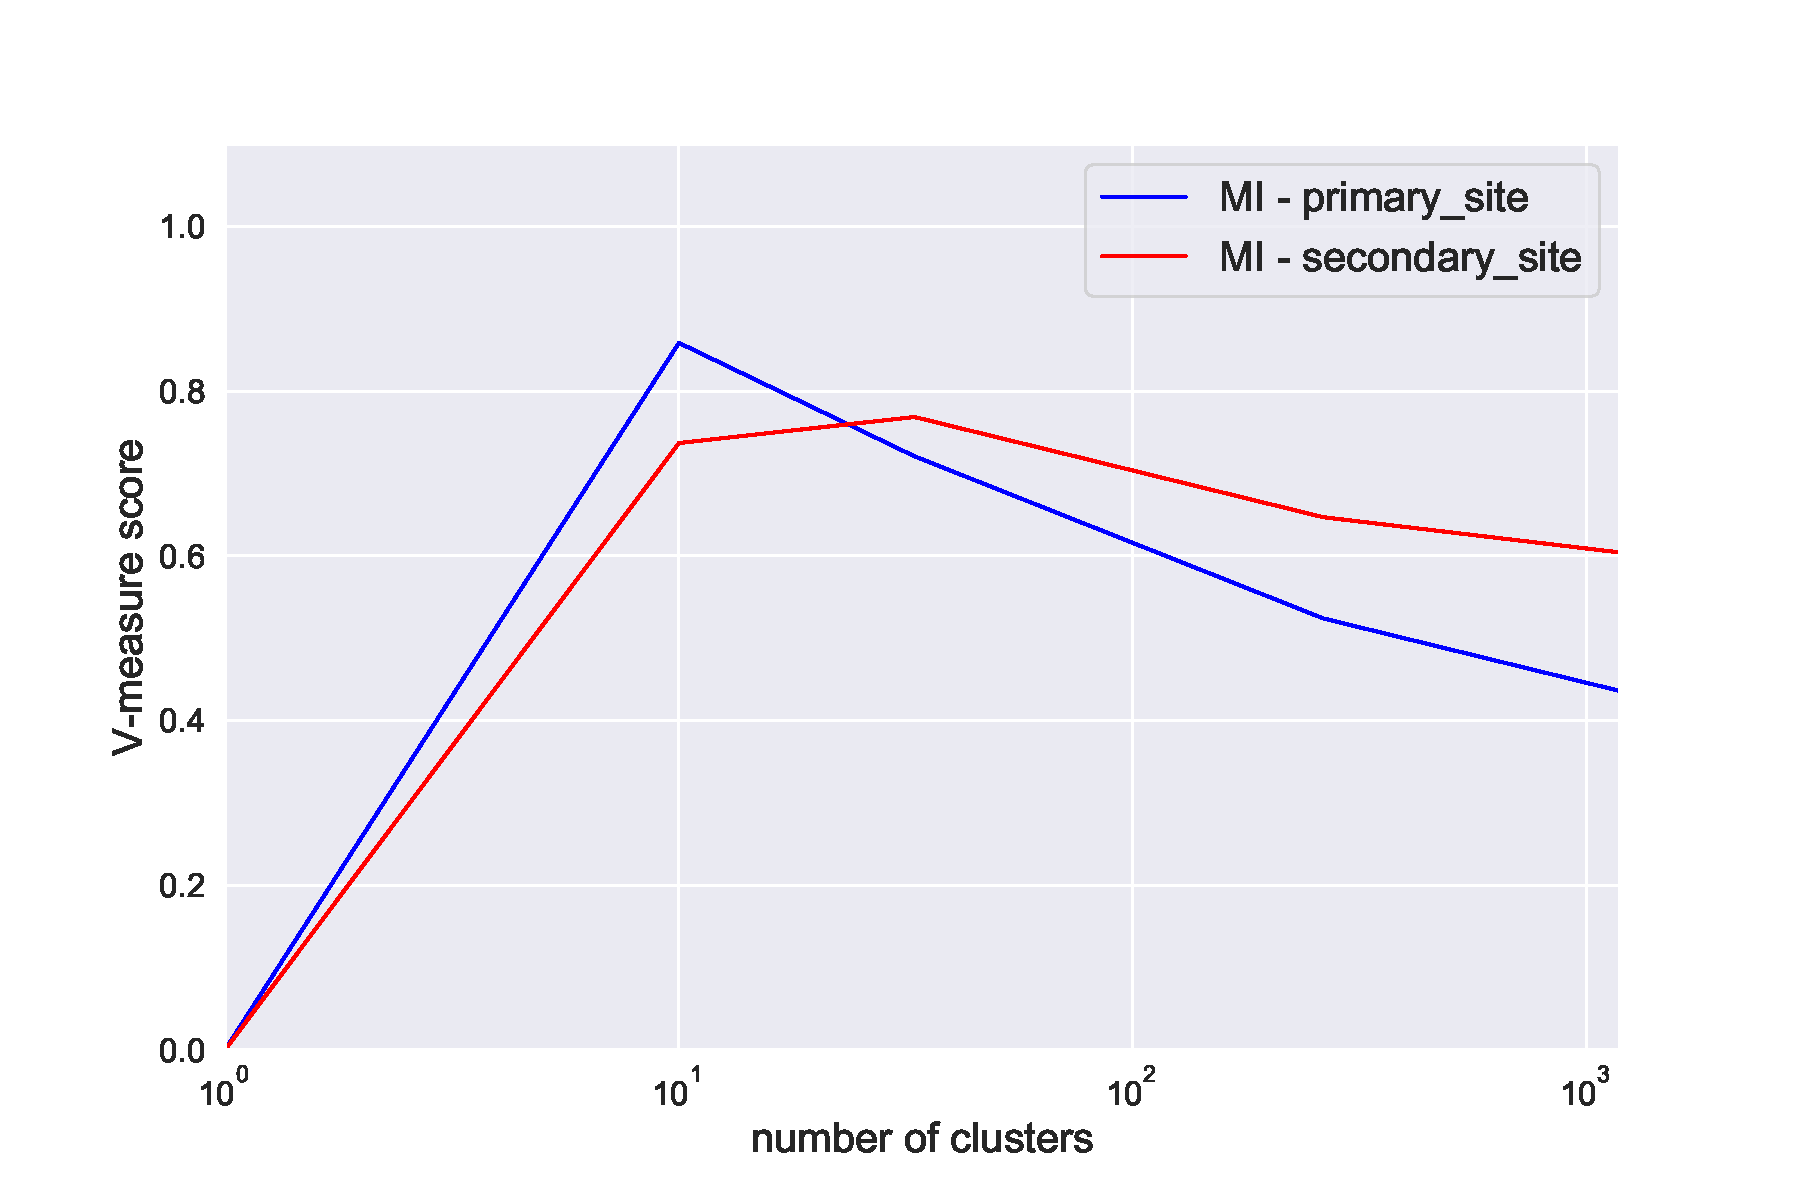
\includegraphics[width=0.9\linewidth]{pictures/topic/gtex/oversigma_10tissue/metric_scores.pdf}
    \caption{Scores across hierarchy}
    \label{fig:topic/gtex/oversigma_10tissue/metric_scores}
\end{figure}
The result is quite good, the maximum score is over $0.8$. Considering that, for example,~\cite{Farver2018} obtained a similar score considering only homogeneity, this is a quite good result. A second interesting fact is that both the tissue label (primary site) and the sub tissue label (secondary site) obtain such a good score, moreover the the secondary site score's peak is at an higher number of clusters coherently with the fact that there is a greater number of sub tissue labels.

In figure~\ref{fig:topic/gtex/oversigma_10tissue/bipartite_rebuild} the relation between the clusters at different layers it is evident.
\begin{figure}[htb!]
    \centering
    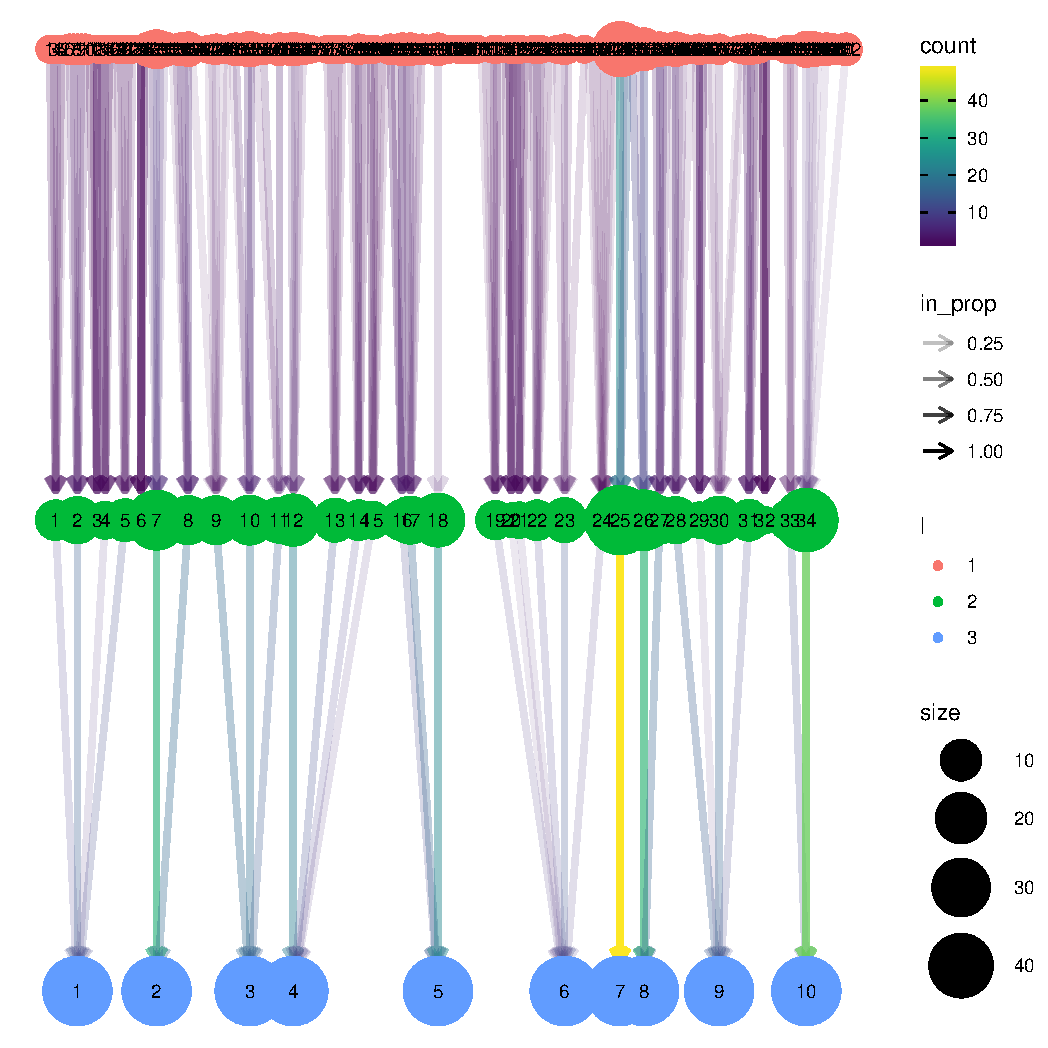
\includegraphics[width=0.8\linewidth]{pictures/topic/gtex/oversigma_10tissue/bipartite_rebuild.pdf}
    \caption{Hierarchy of the files' nodes}
    \label{fig:topic/gtex/oversigma_10tissue/bipartite_rebuild}
\end{figure}

\clearpage
In figure~\ref{fig:topic/gtex/oversigma_10tissue/clustercomposition_l3_primary_site} each column is a cluster and each colour is a tissue of the dataset. It is evident that the majority of the tissue are identified: the first, second, fifth, sixth, eighth and tenth columns are fully and uniformly coloured of the same colour. These corresponds to an identification of brain, blood, lung, testis and bladder.
\begin{figure}[htb!]
    \centering
    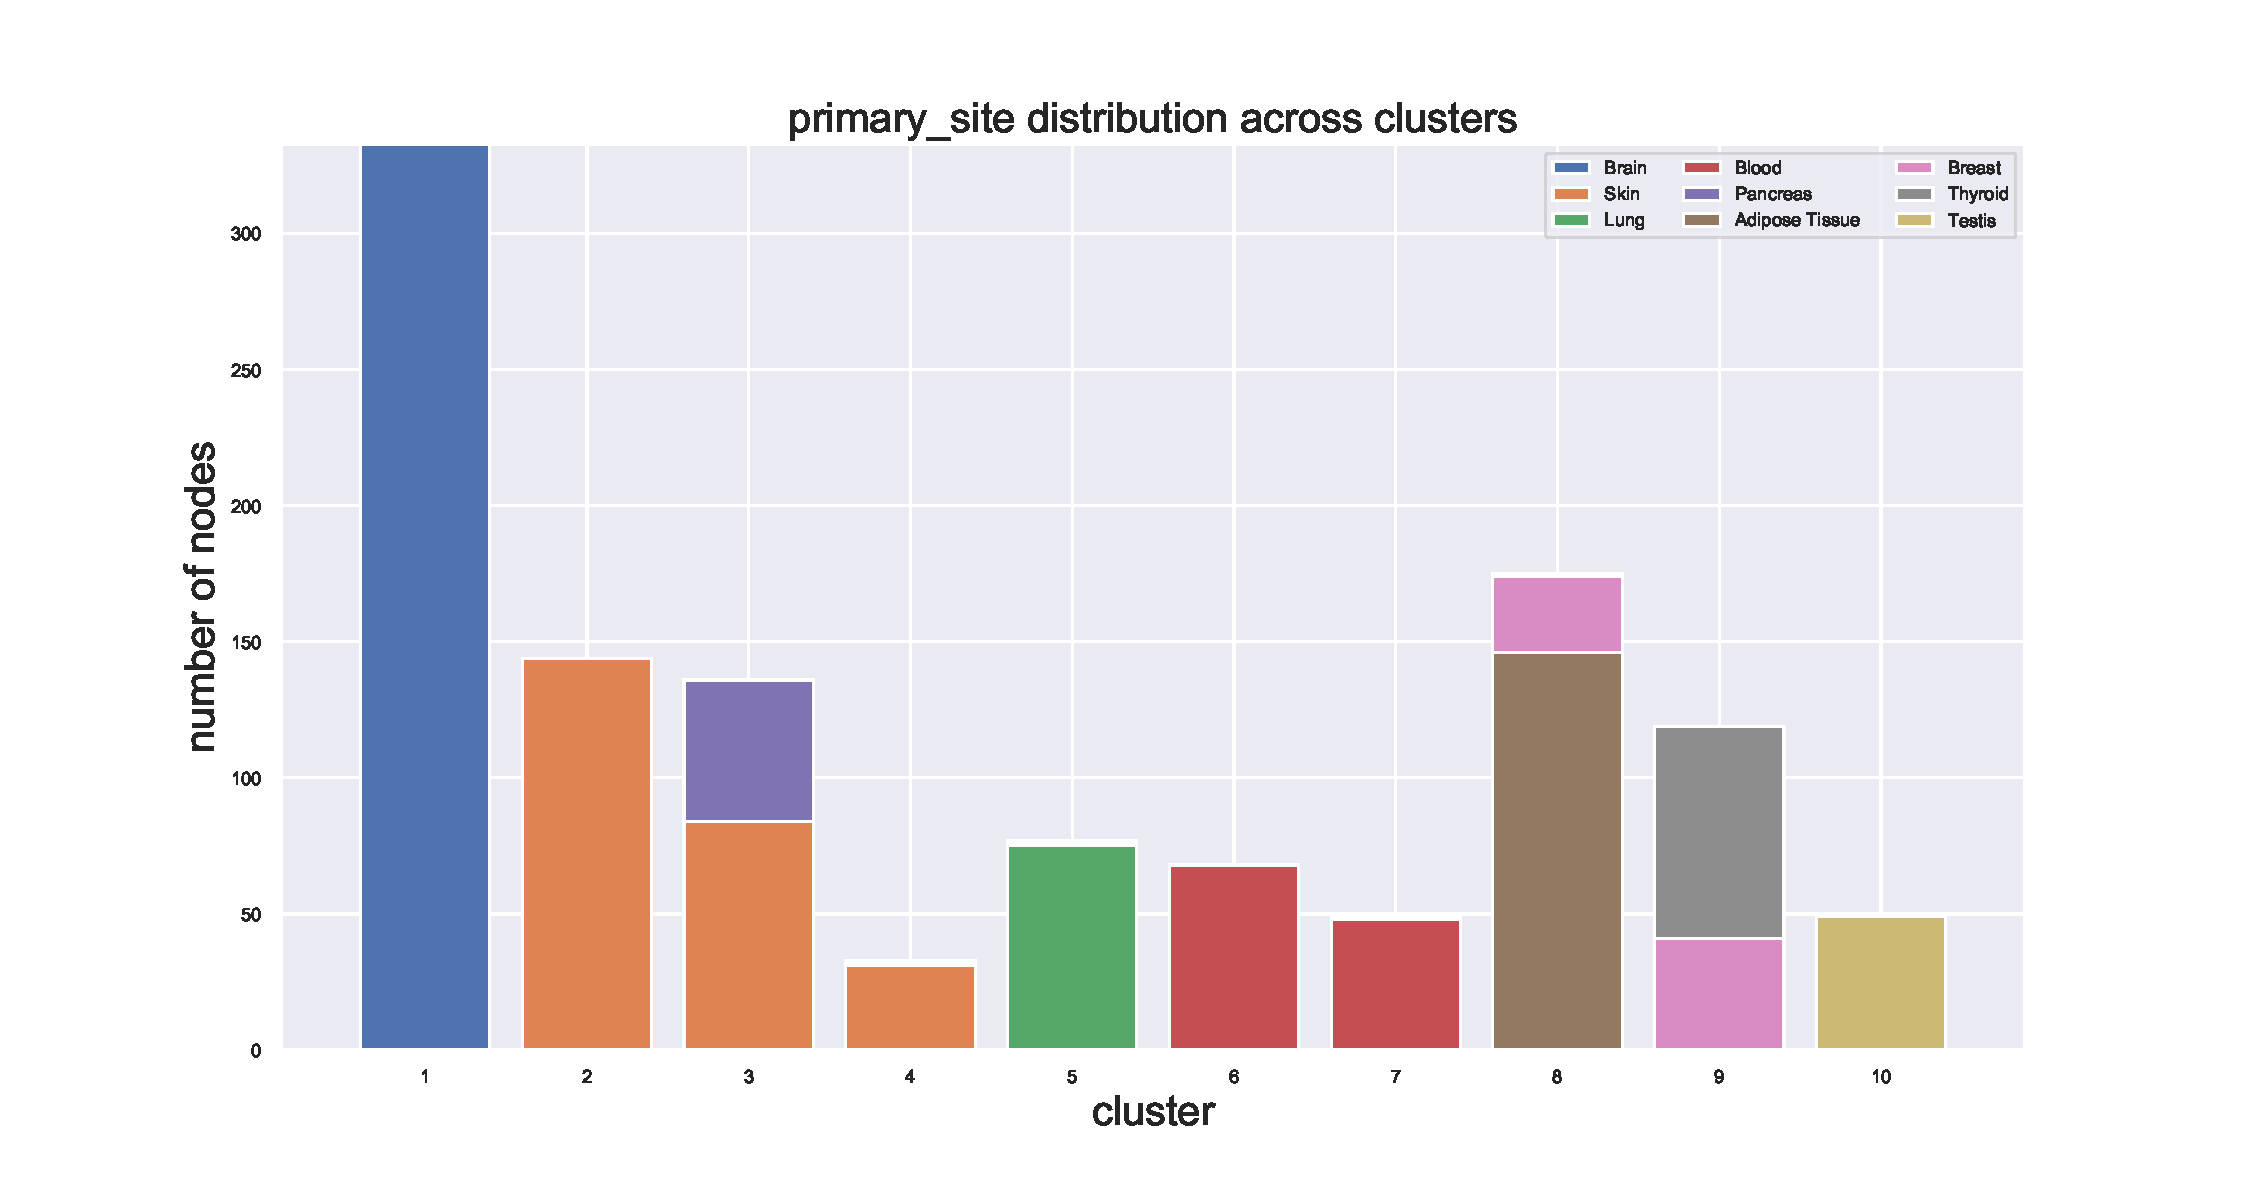
\includegraphics[width=0.9\linewidth]{pictures/topic/gtex/oversigma_10tissue/clustercomposition_l3_primary_site.pdf}
    \caption{Caption}
    \label{fig:topic/gtex/oversigma_10tissue/clustercomposition_l3_primary_site}
\end{figure}
A normalised representation of the same clusters the result is still quite interesting and the homogeneity of the clusters is more evident.
\begin{figure}[htb!]
    \centering
    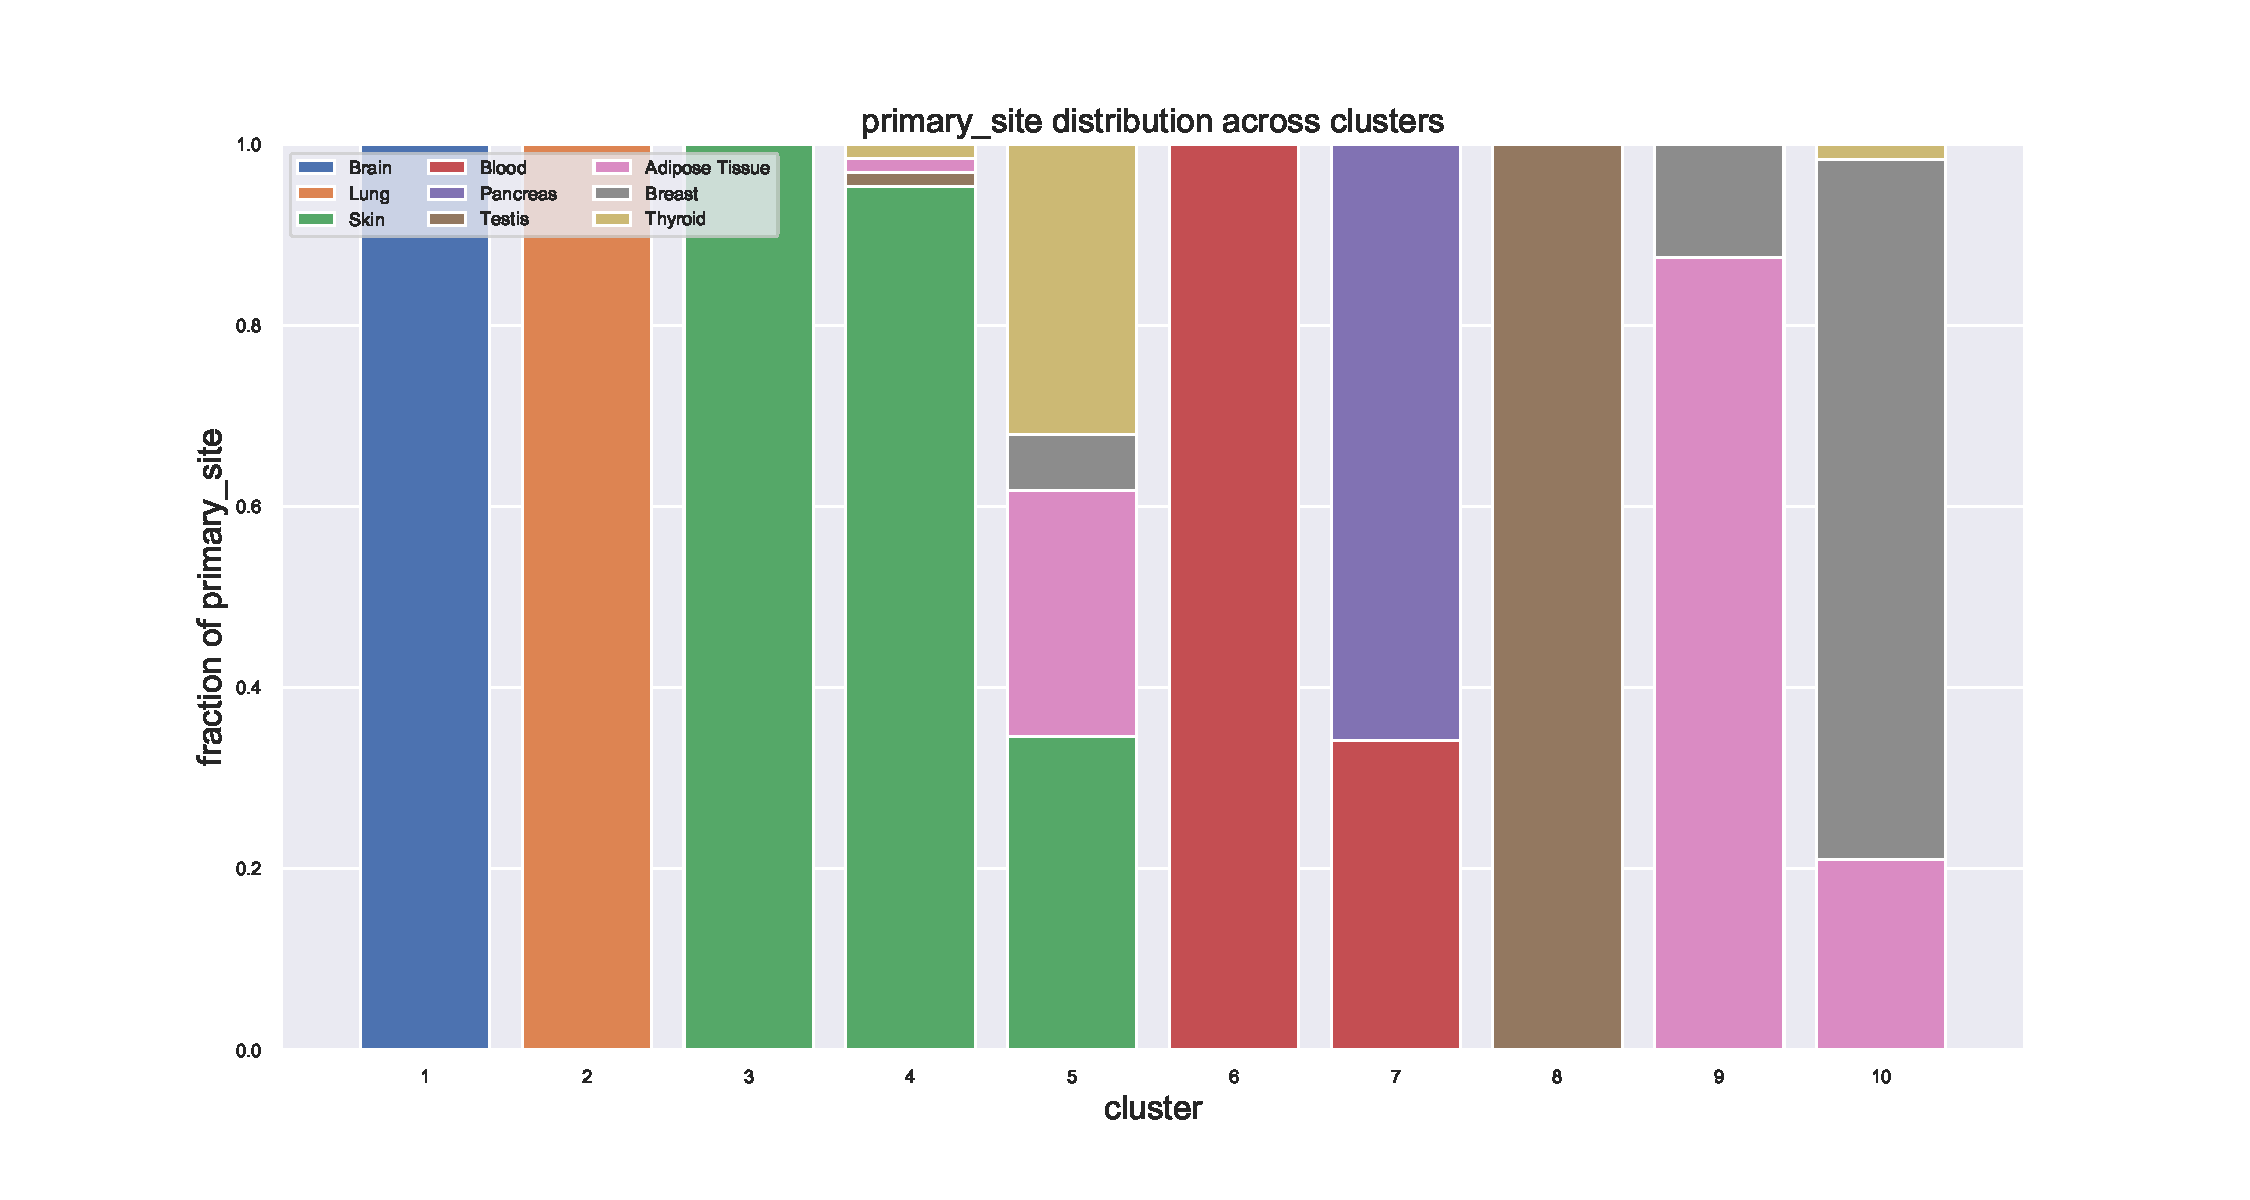
\includegraphics[width=0.9\linewidth]{pictures/topic/gtex/oversigma_10tissue/fraction_clustercomposition_l3_primary_site.pdf}
    \caption{Caption}
    \label{fig:topic/gtex/oversigma_10tissue/fraction_clustercomposition_l3_primary_site}
\end{figure}
Going forward in the hierarchy and looking at a layer with more cluster the result, shown in figure~\ref{fig:topic/gtex/oversigma_10tissue/fraction_clustercomposition_l2_primary_site}, demonstrates that at this point all the the tissues are separated and each cluster is representative of a tissue.
\begin{figure}[htb!]
    \centering
    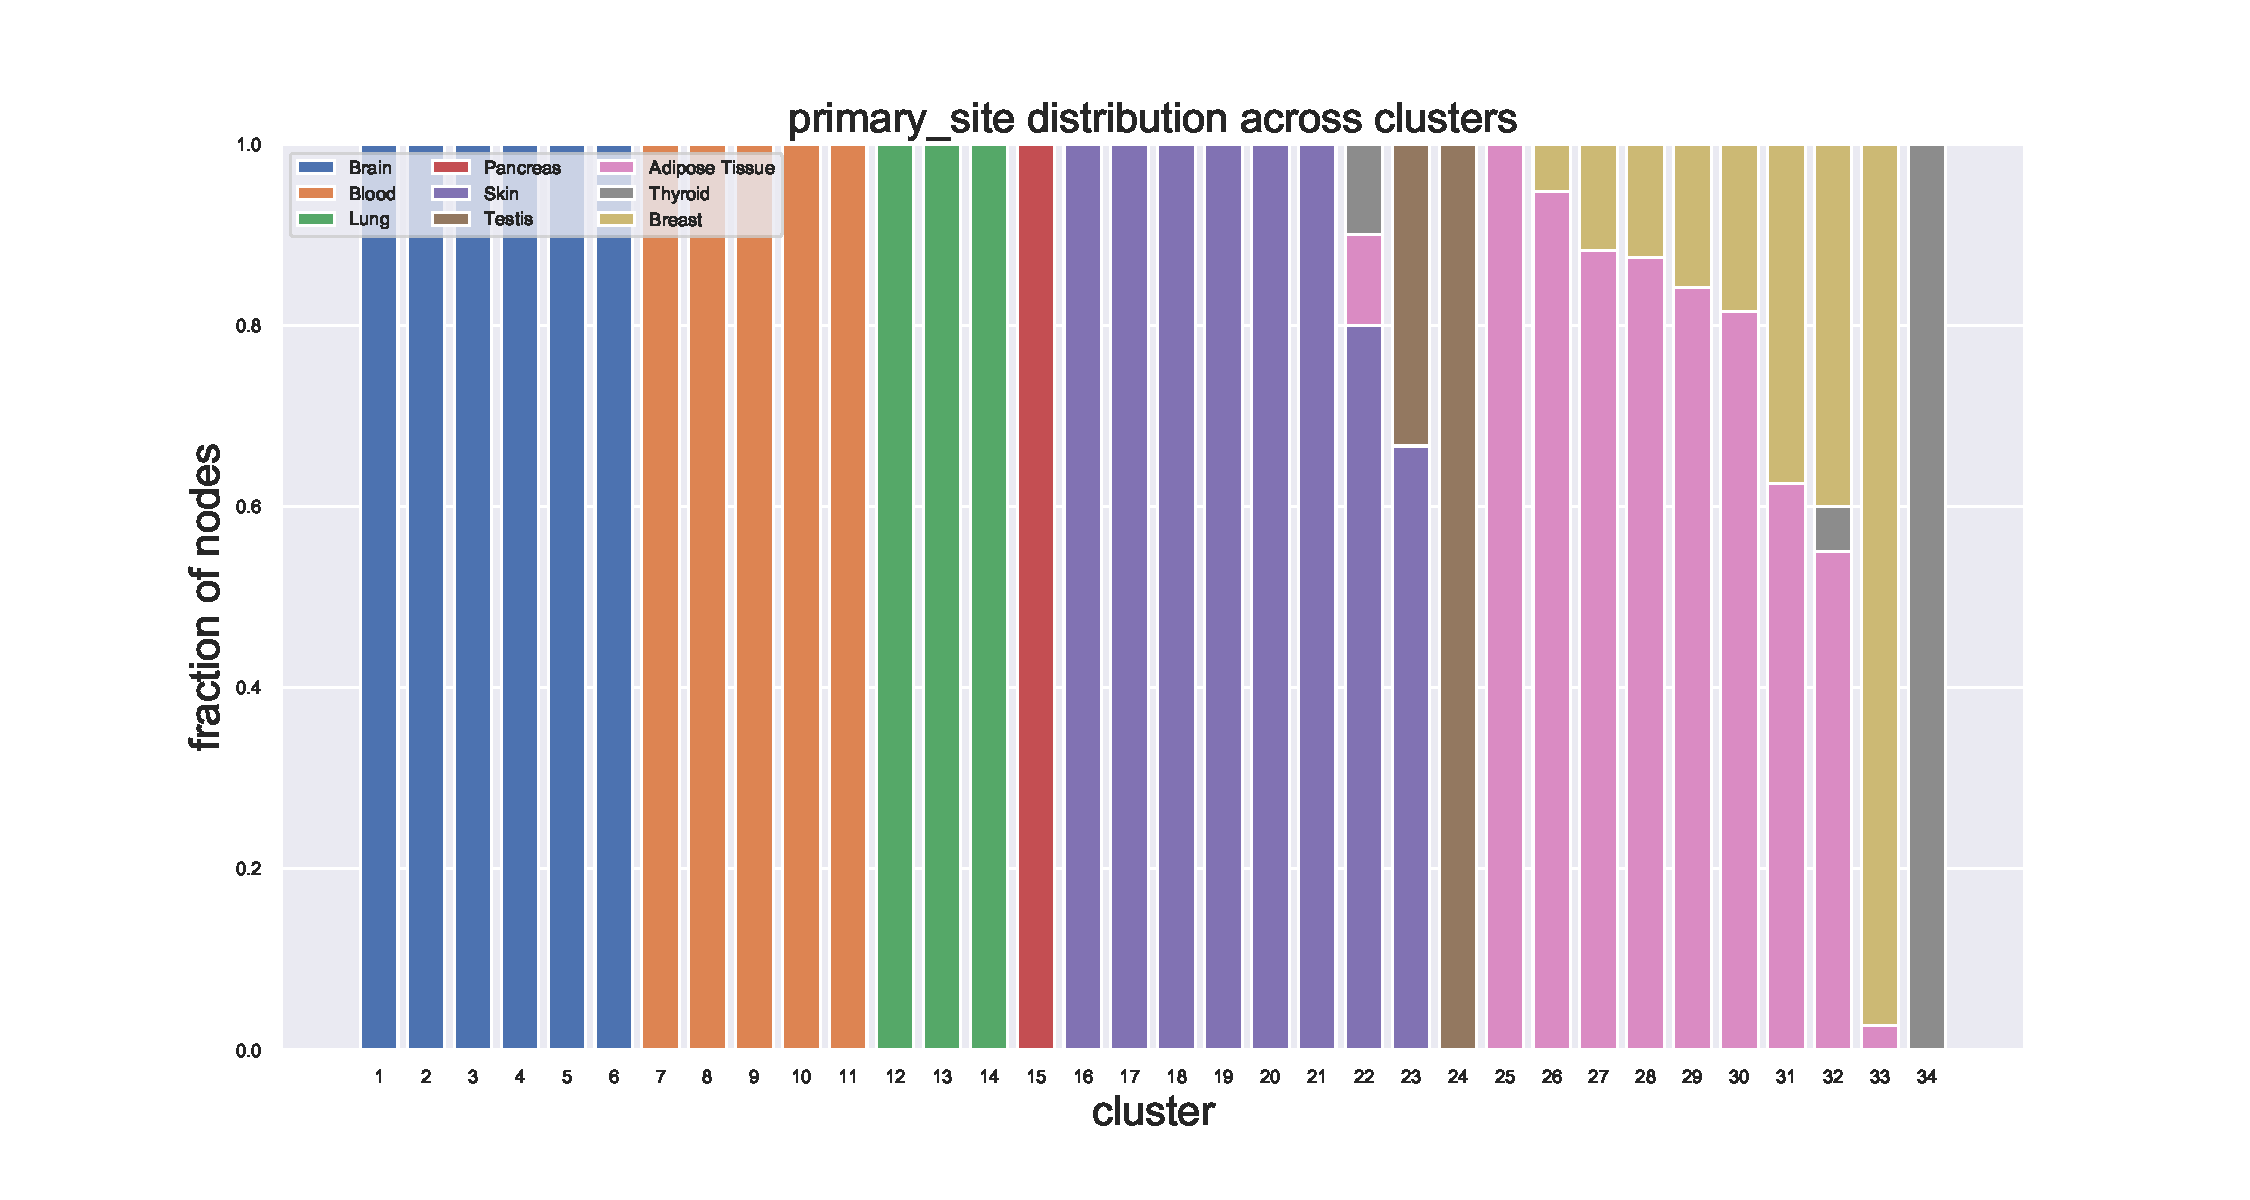
\includegraphics[width=0.9\linewidth]{pictures/topic/gtex/oversigma_10tissue/fraction_clustercomposition_l2_primary_site.pdf}
    \caption{Caption}
    \label{fig:topic/gtex/oversigma_10tissue/fraction_clustercomposition_l2_primary_site}
\end{figure}
Even looking at sub-tissues the results is quite good. It is not always easy to separate all the sub-parts of brain, nevertheless the cerebellum is well identified and blood is distinguished in whole blood and lymphocytes.
\begin{figure}[htb!]
    \centering
    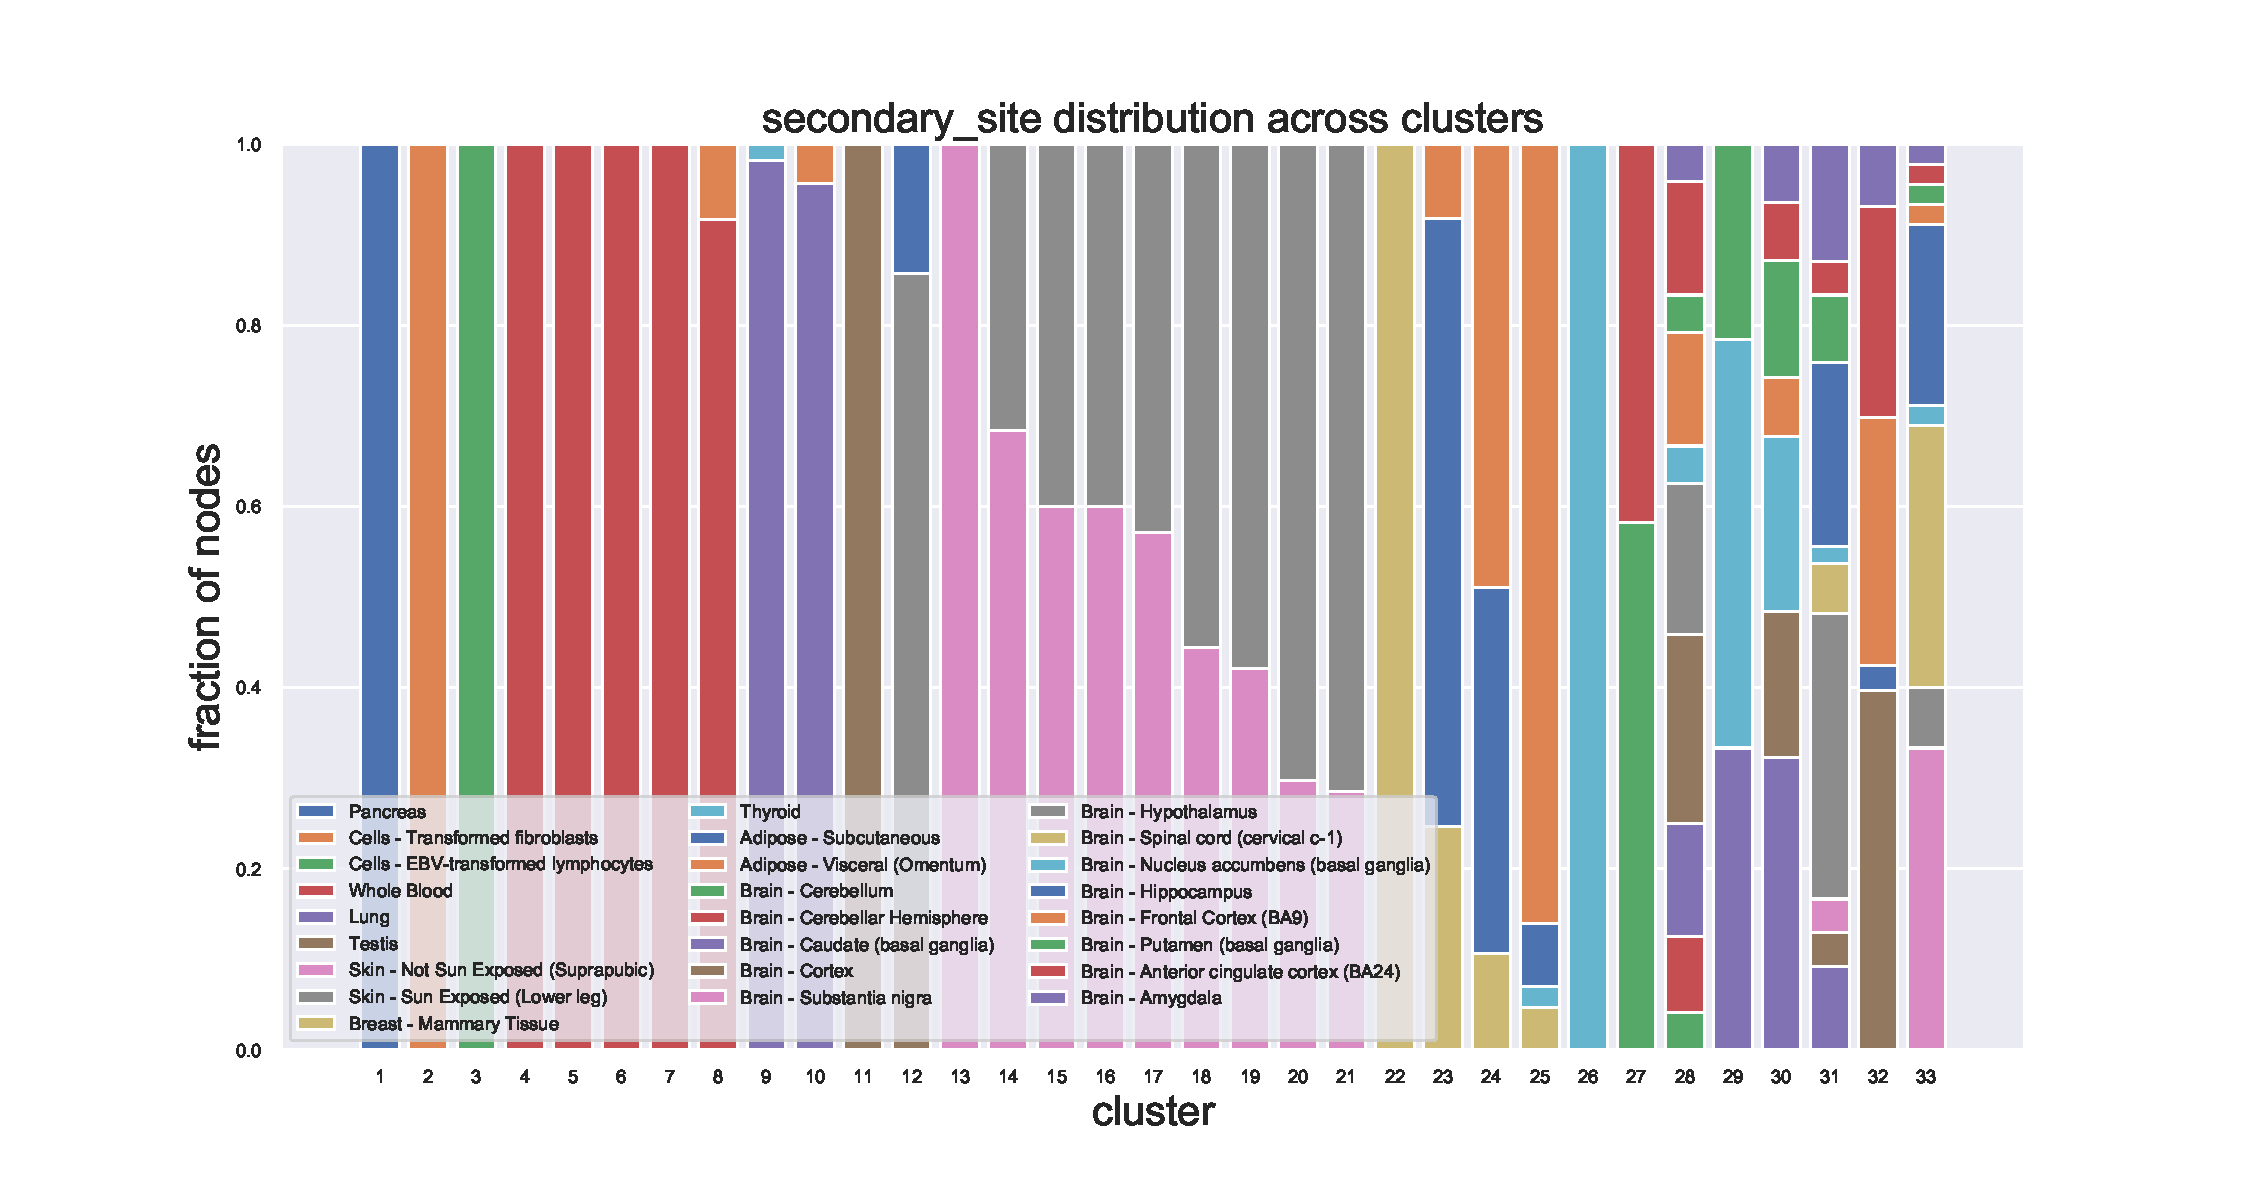
\includegraphics[width=0.9\linewidth]{pictures/topic/gtex/oversigma_10tissue/fraction_clustercomposition_l2_secondary_site.pdf}
    \caption{Caption}
    \label{fig:topic/gtex/oversigma_10tissue/fraction_clustercomposition_l2_secondary_site}
\end{figure}

All the results described in the previous pictures are quite qualitative. To have a more objective and mathematical measure of the success of the algorithm it is possible to measure the fraction of the most representative label in each cluster $k$
\[
max_{l\in labels}\left(\frac{n_{l k}}{n_k}\right)
\]
with $n_{l k}$ is the numbers of nodes labelled $l$ in cluster $k$ and $n_k$ is the number of nodes in cluster $k$. This is represented in figure~\ref{fig:gtex/oversigma_10tissue/shuffledcluster_maximum_l2_primary_site} for the level where the V-measure is maximised (best results are expected here).
\begin{figure}[htb!]
    \centering
    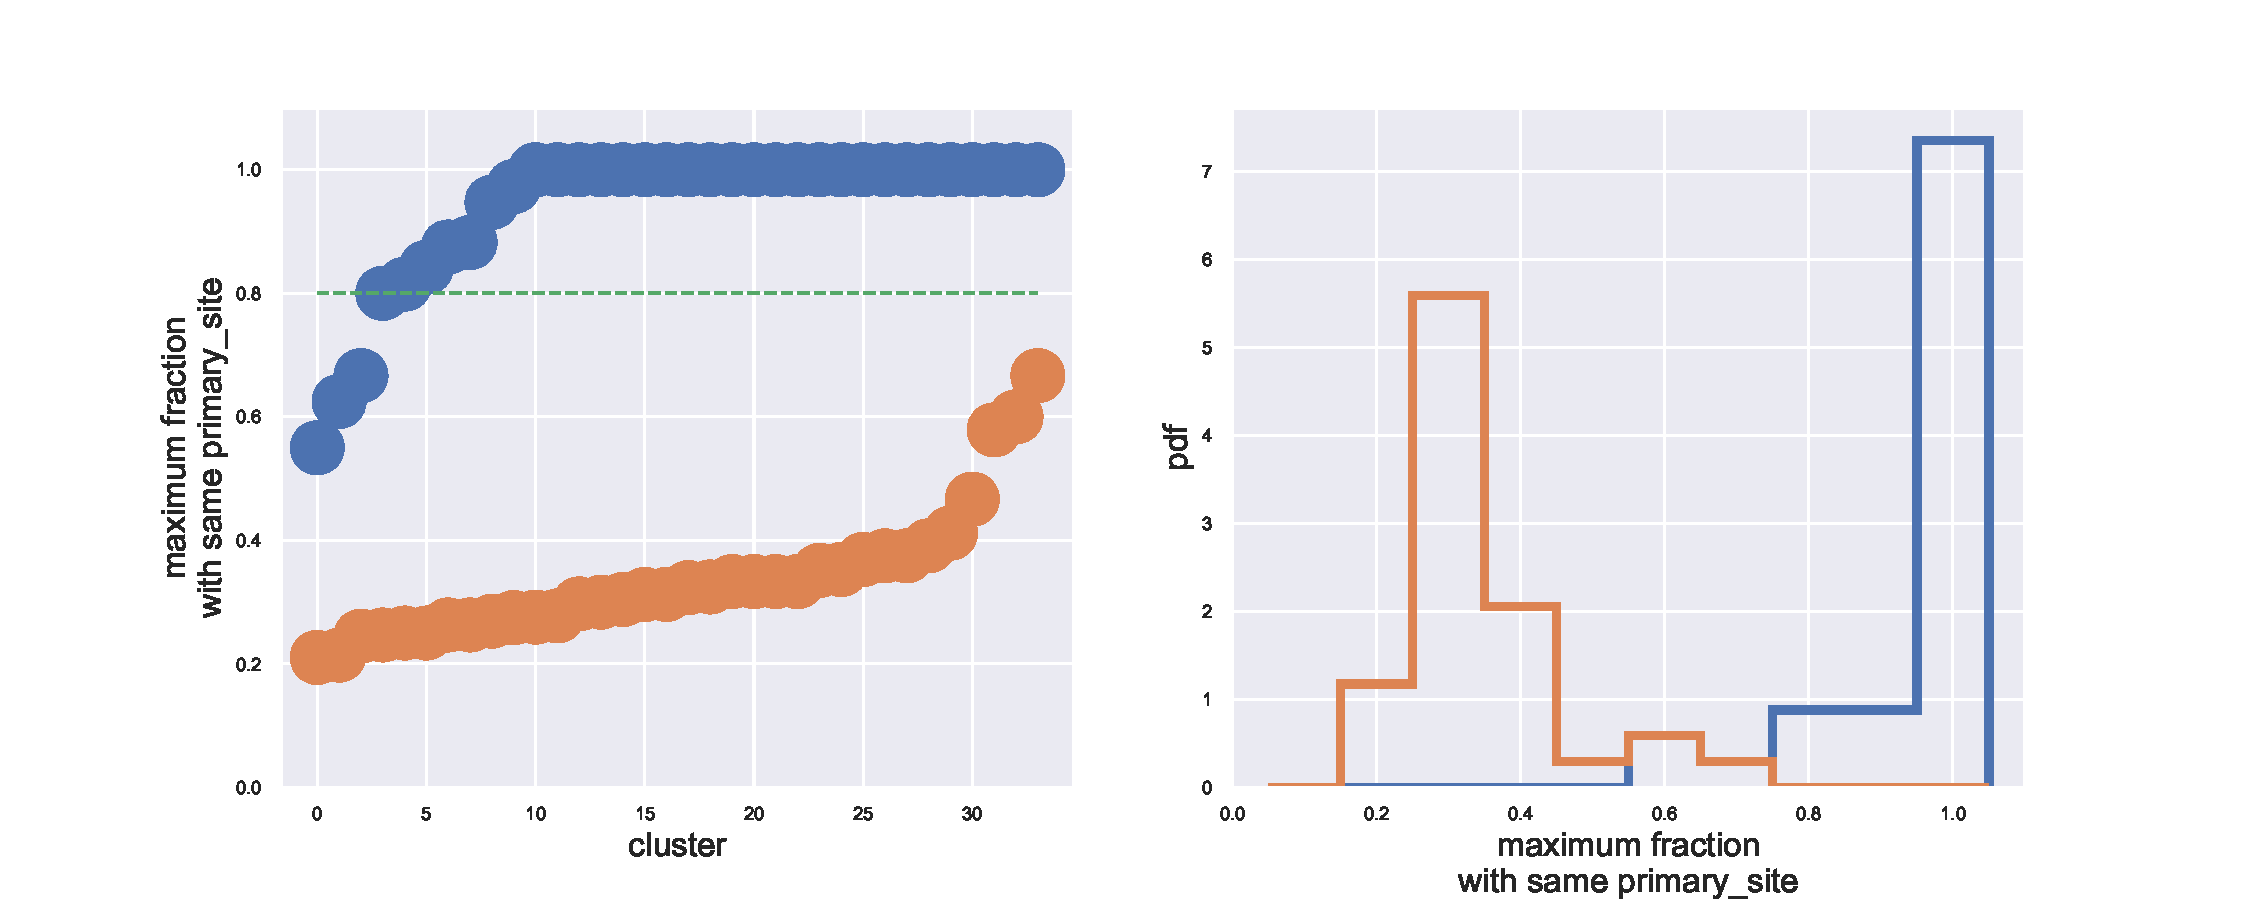
\includegraphics[width=0.9\linewidth]{pictures/topic/gtex/oversigma_10tissue/shuffledcluster_maximum_l2_primary_site.pdf}
    \caption{Caption}
    \label{fig:gtex/oversigma_10tissue/shuffledcluster_maximum_l2_primary_site}
\end{figure}
In figure~\ref{fig:topic/gtex/oversigma_10tissue/shuffledcluster_maximum*}
\begin{figure}[htb!]
    \centering
    \begin{minipage}{0.45\textwidth}
    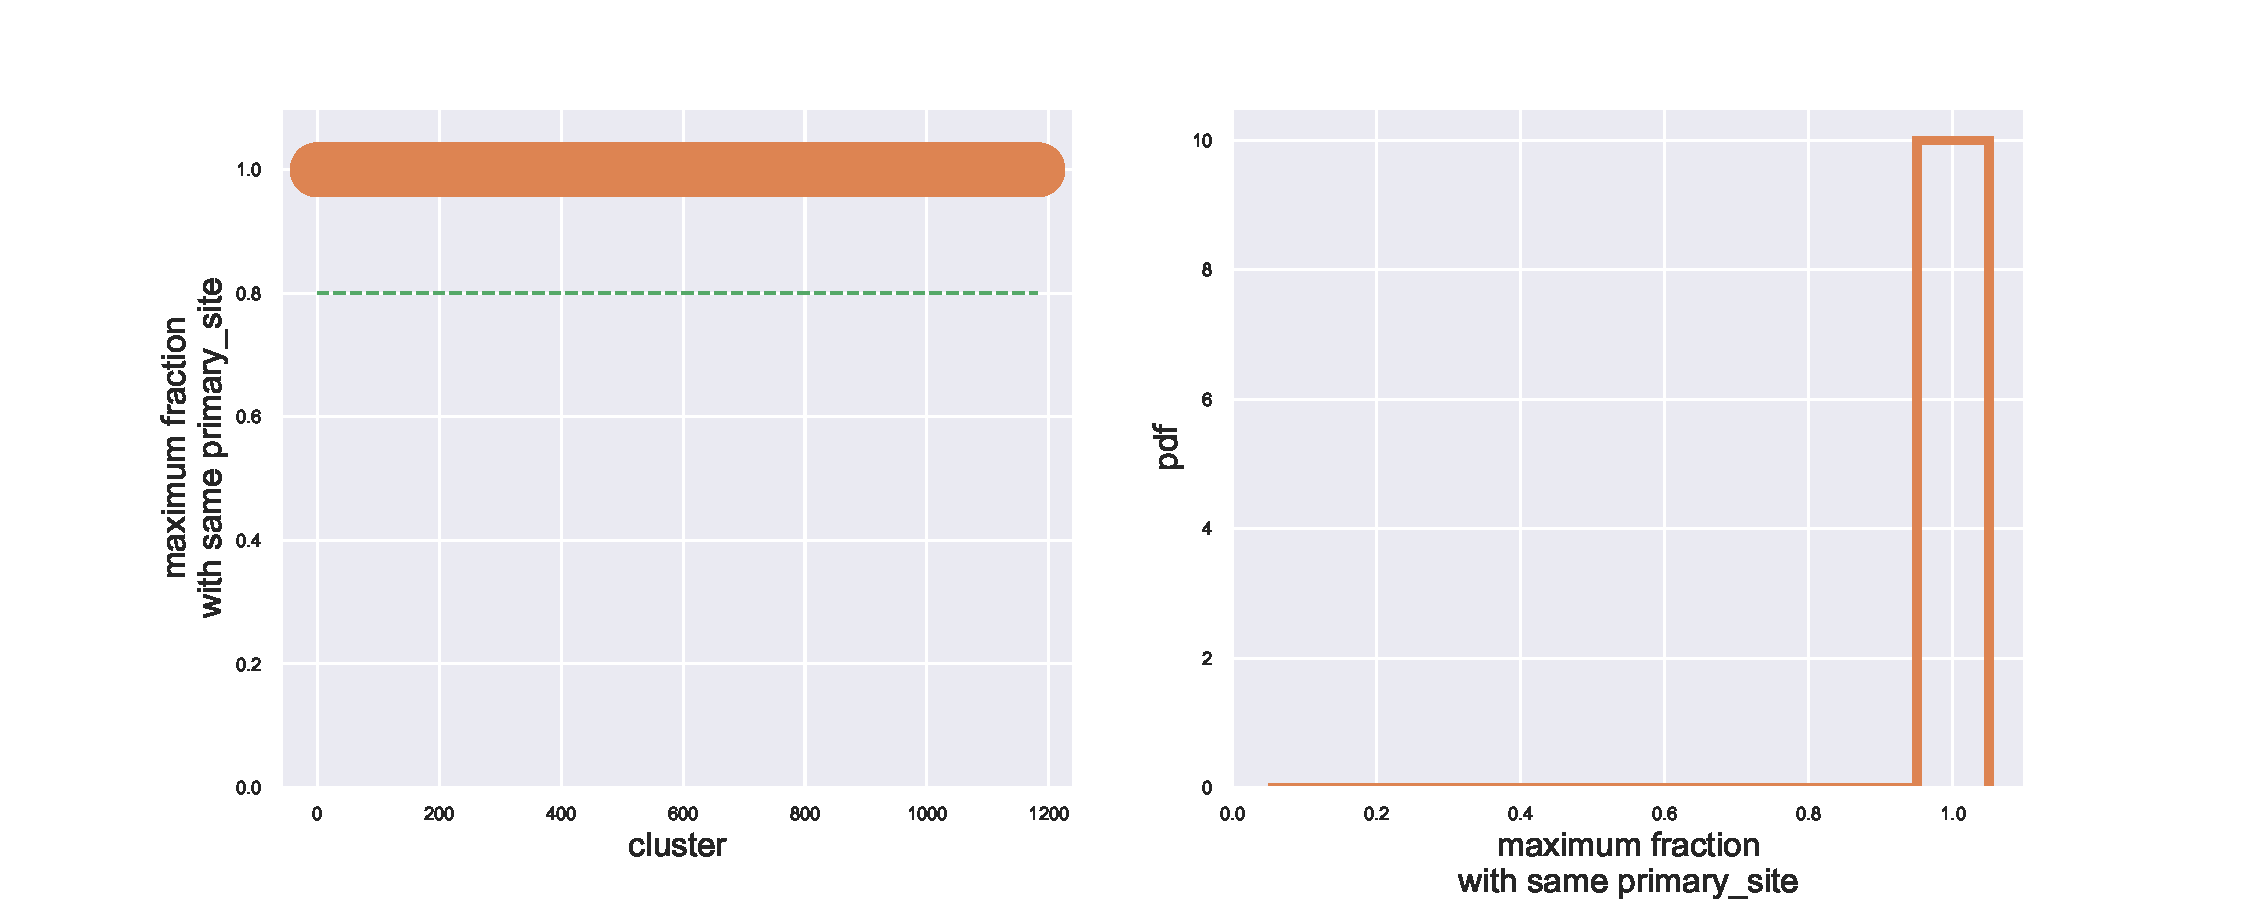
\includegraphics[width=0.9\linewidth]{pictures/topic/gtex/oversigma_10tissue/shuffledcluster_maximum_l0_primary_site.pdf}
    \end{minipage}
    \hspace{3mm}
    \begin{minipage}{0.45\textwidth}
    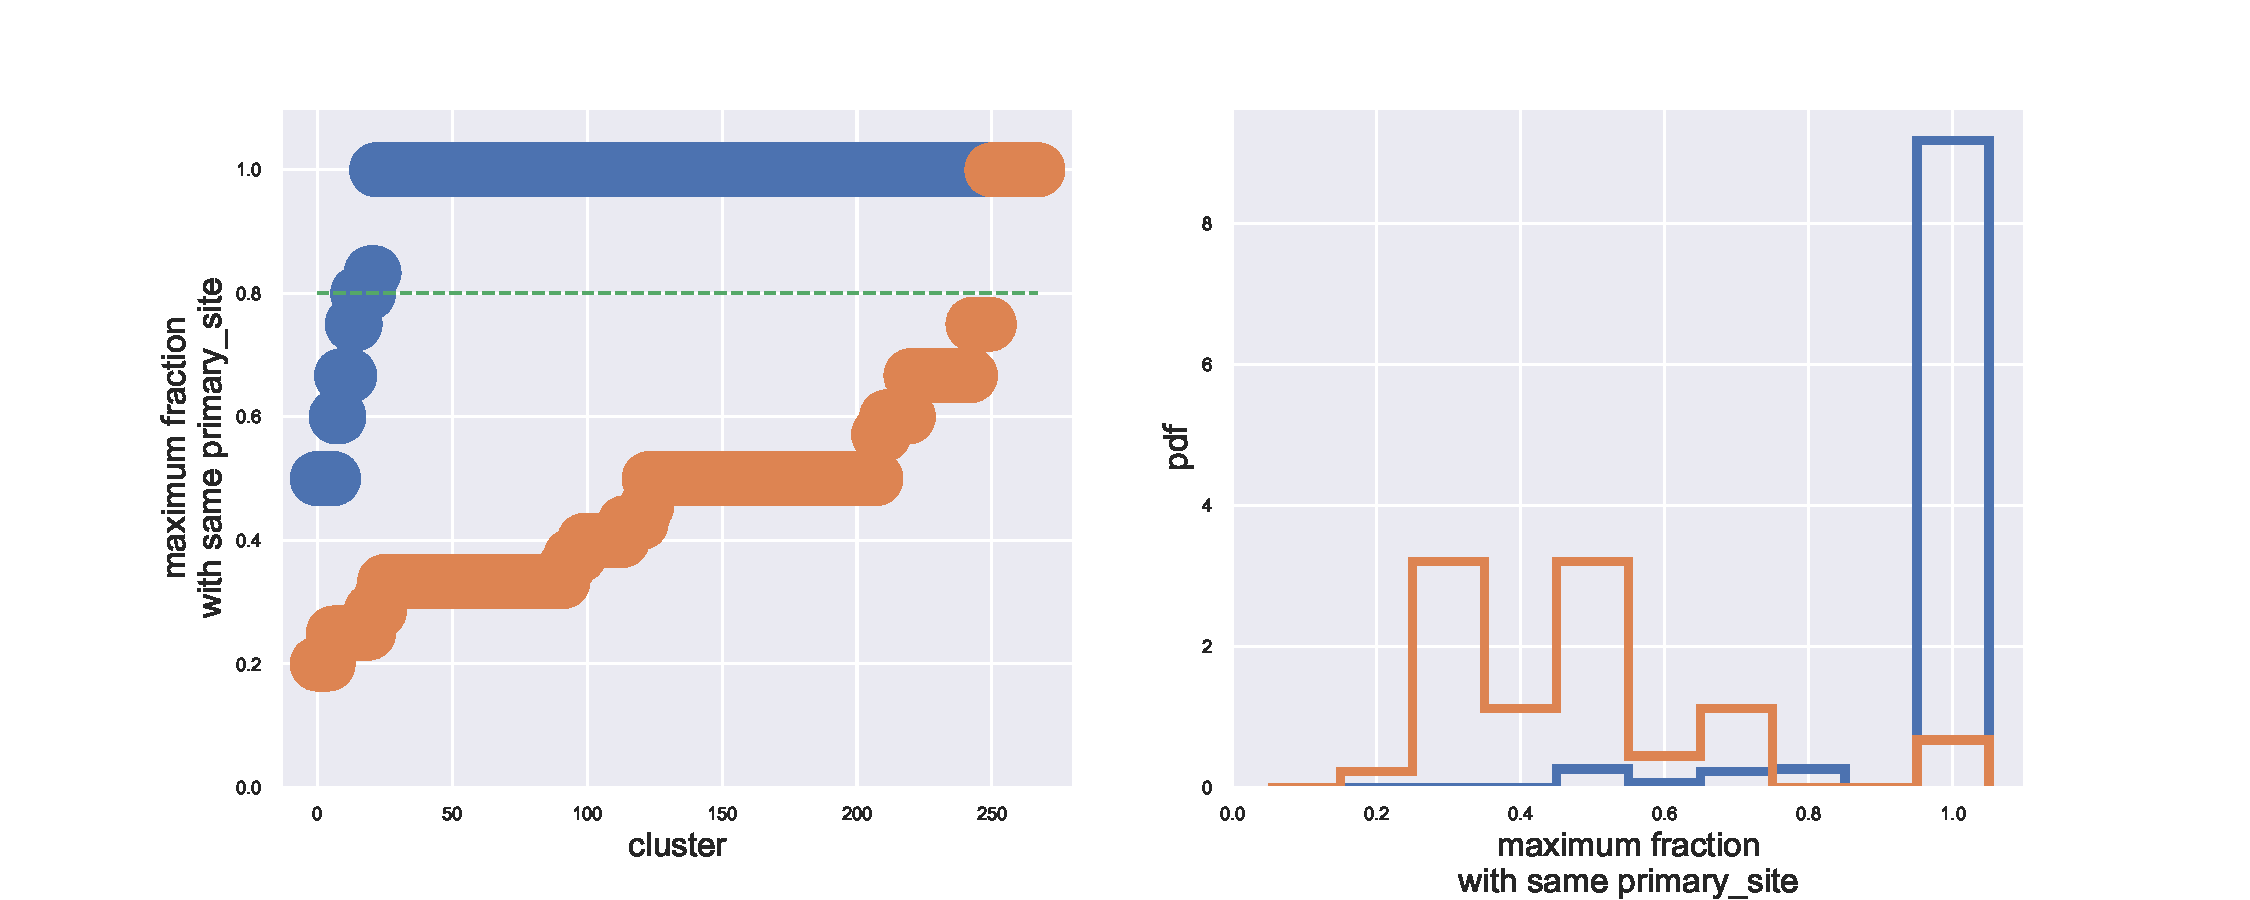
\includegraphics[width=0.9\linewidth]{pictures/topic/gtex/oversigma_10tissue/shuffledcluster_maximum_l1_primary_site.pdf}
    \end{minipage}
    \\
    \begin{minipage}{0.45\textwidth}
    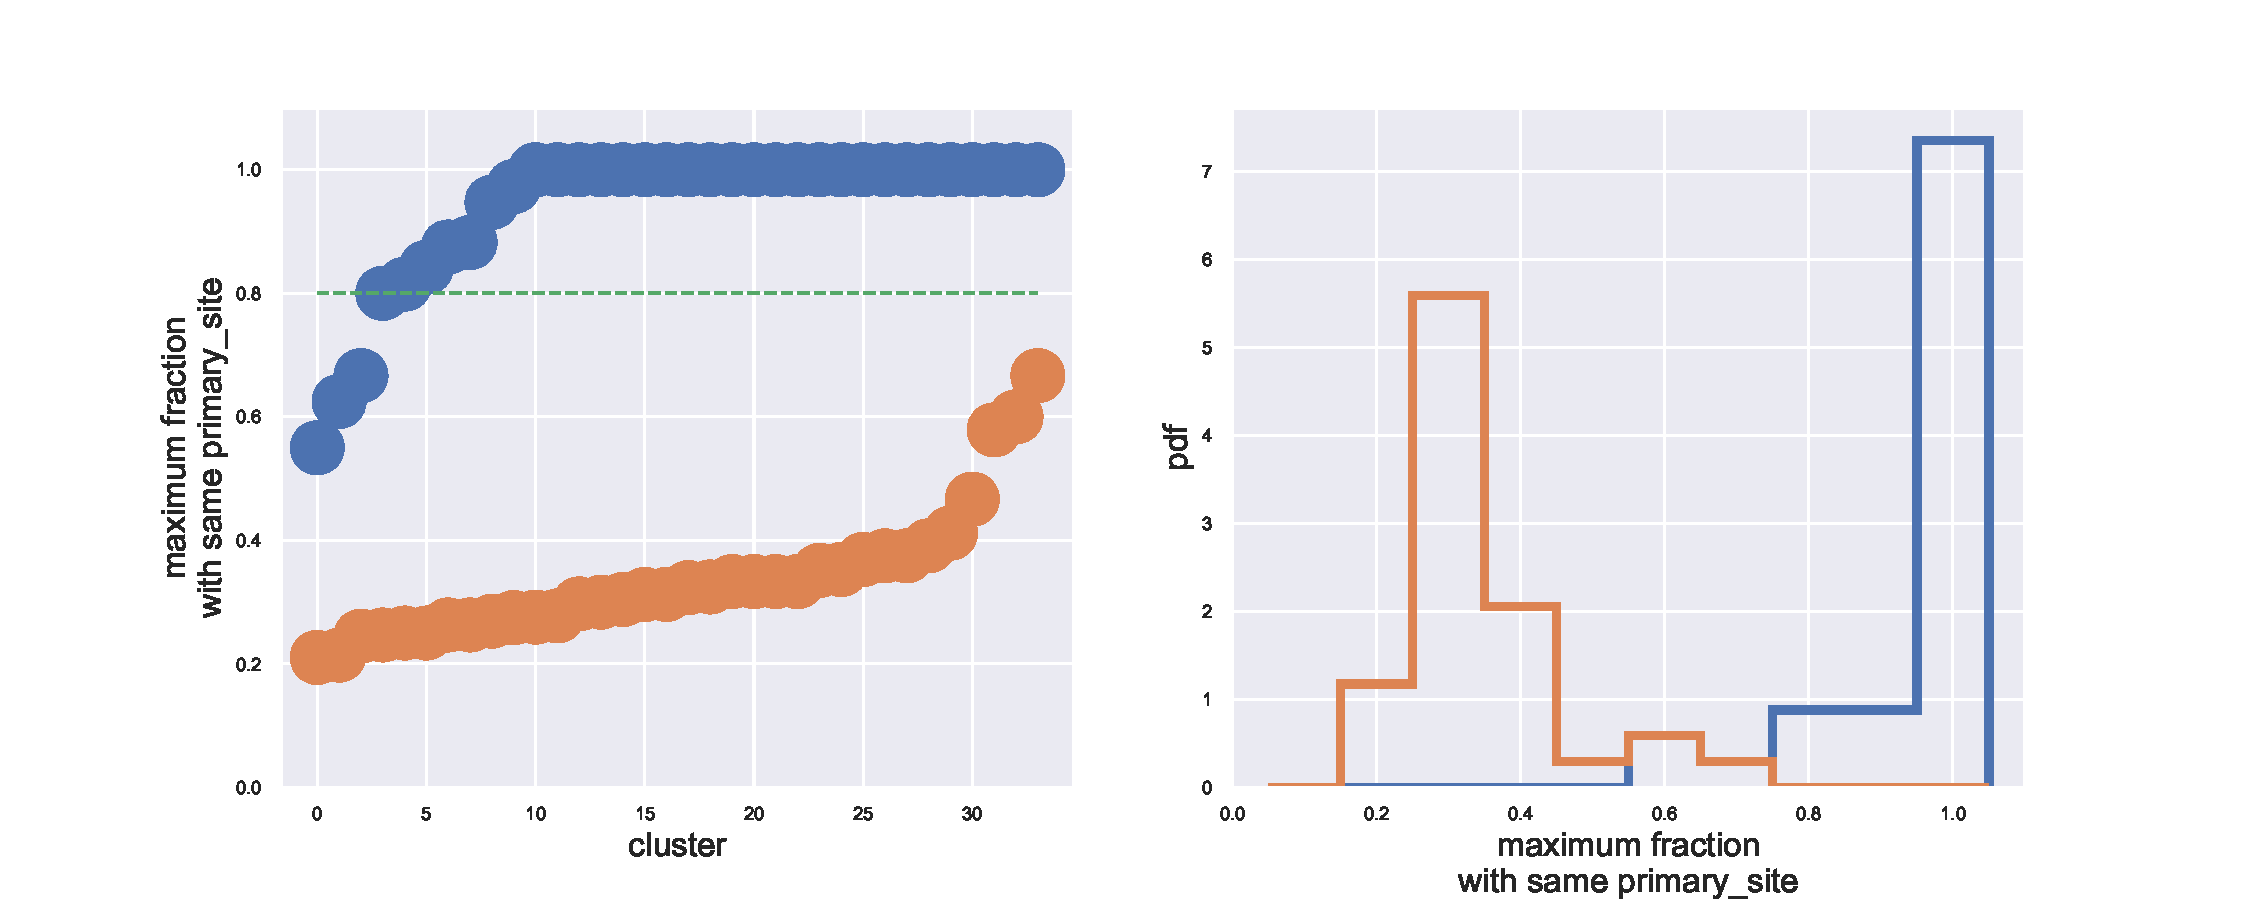
\includegraphics[width=0.9\linewidth]{pictures/topic/gtex/oversigma_10tissue/shuffledcluster_maximum_l2_primary_site.pdf}
    \end{minipage}
    \hspace{3mm}
    \begin{minipage}{0.45\textwidth}
    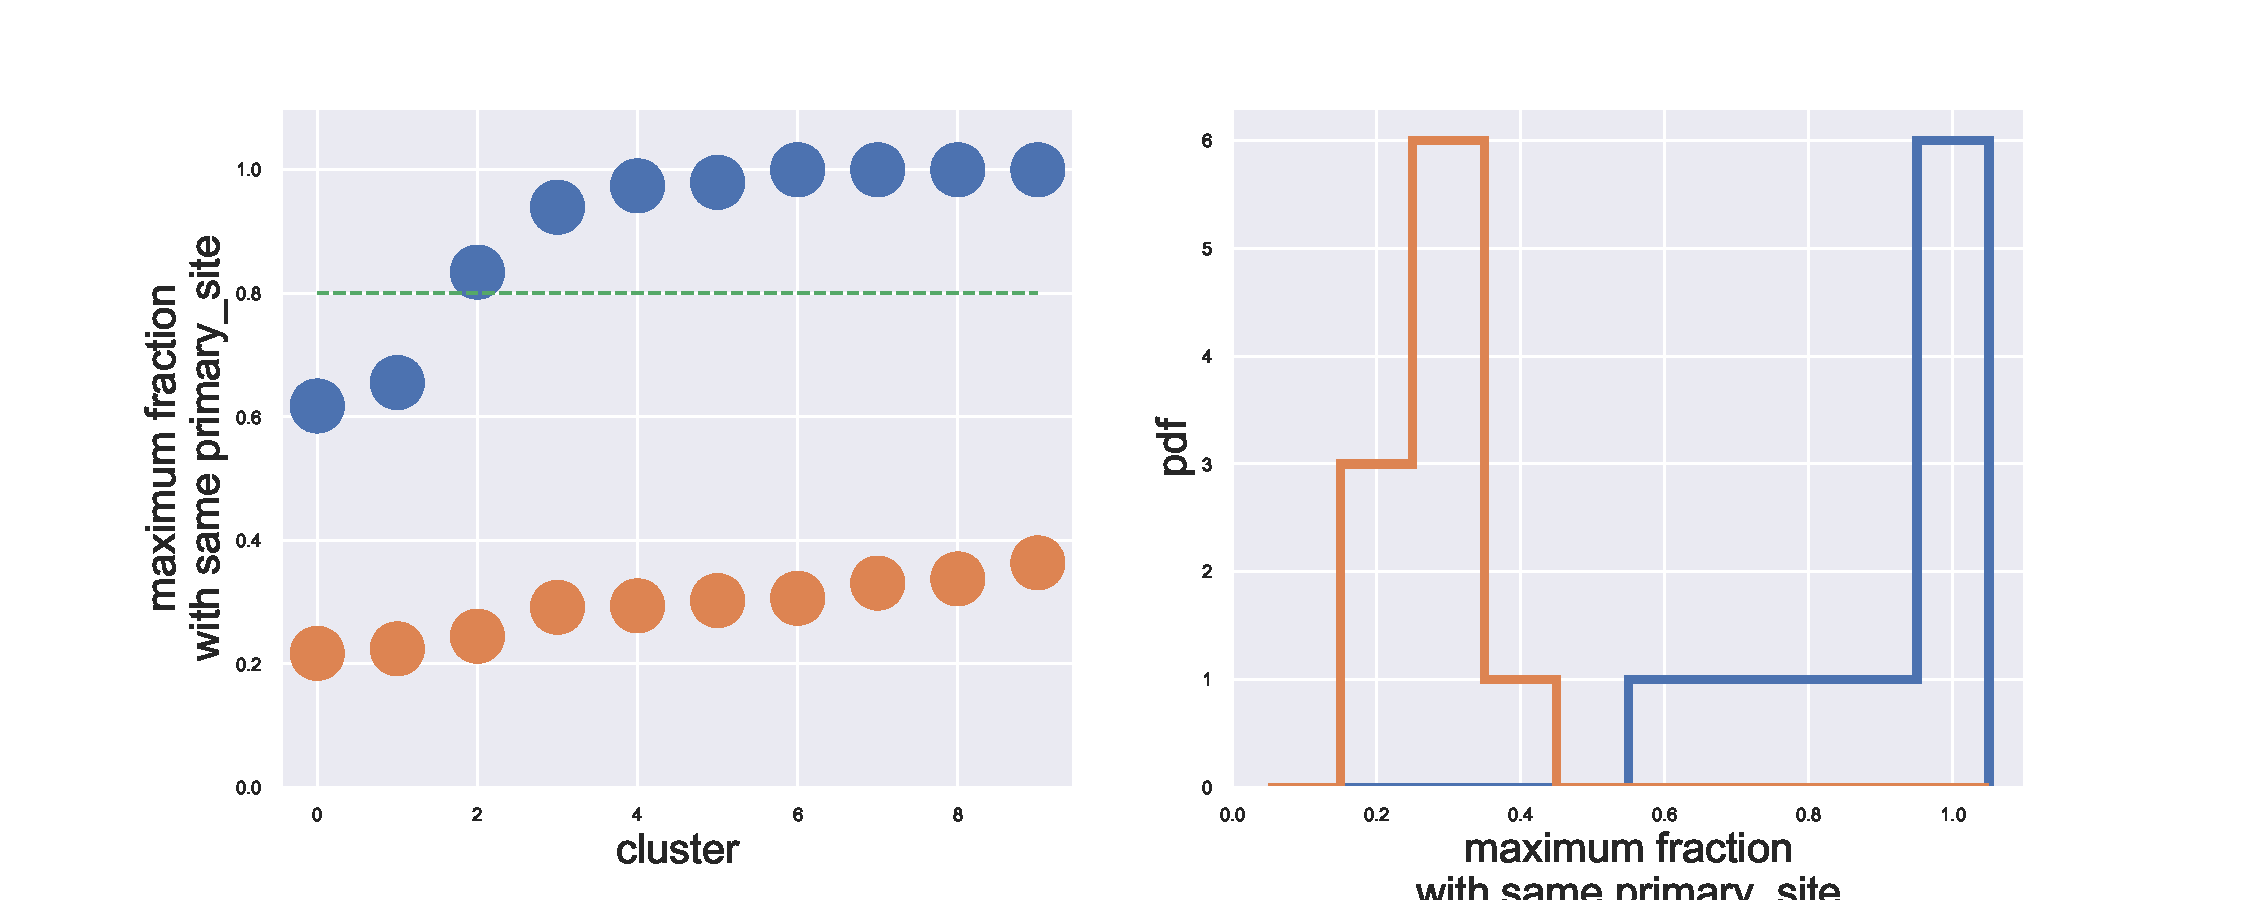
\includegraphics[width=0.9\linewidth]{pictures/topic/gtex/oversigma_10tissue/shuffledcluster_maximum_l3_primary_site.pdf}
    \end{minipage}
    \label{fig:topic/gtex/oversigma_10tissue/shuffledcluster_maximum*}
    \caption{Beahviour across the hierarchy}
\end{figure}

\begin{figure}[htb!]
    \centering
    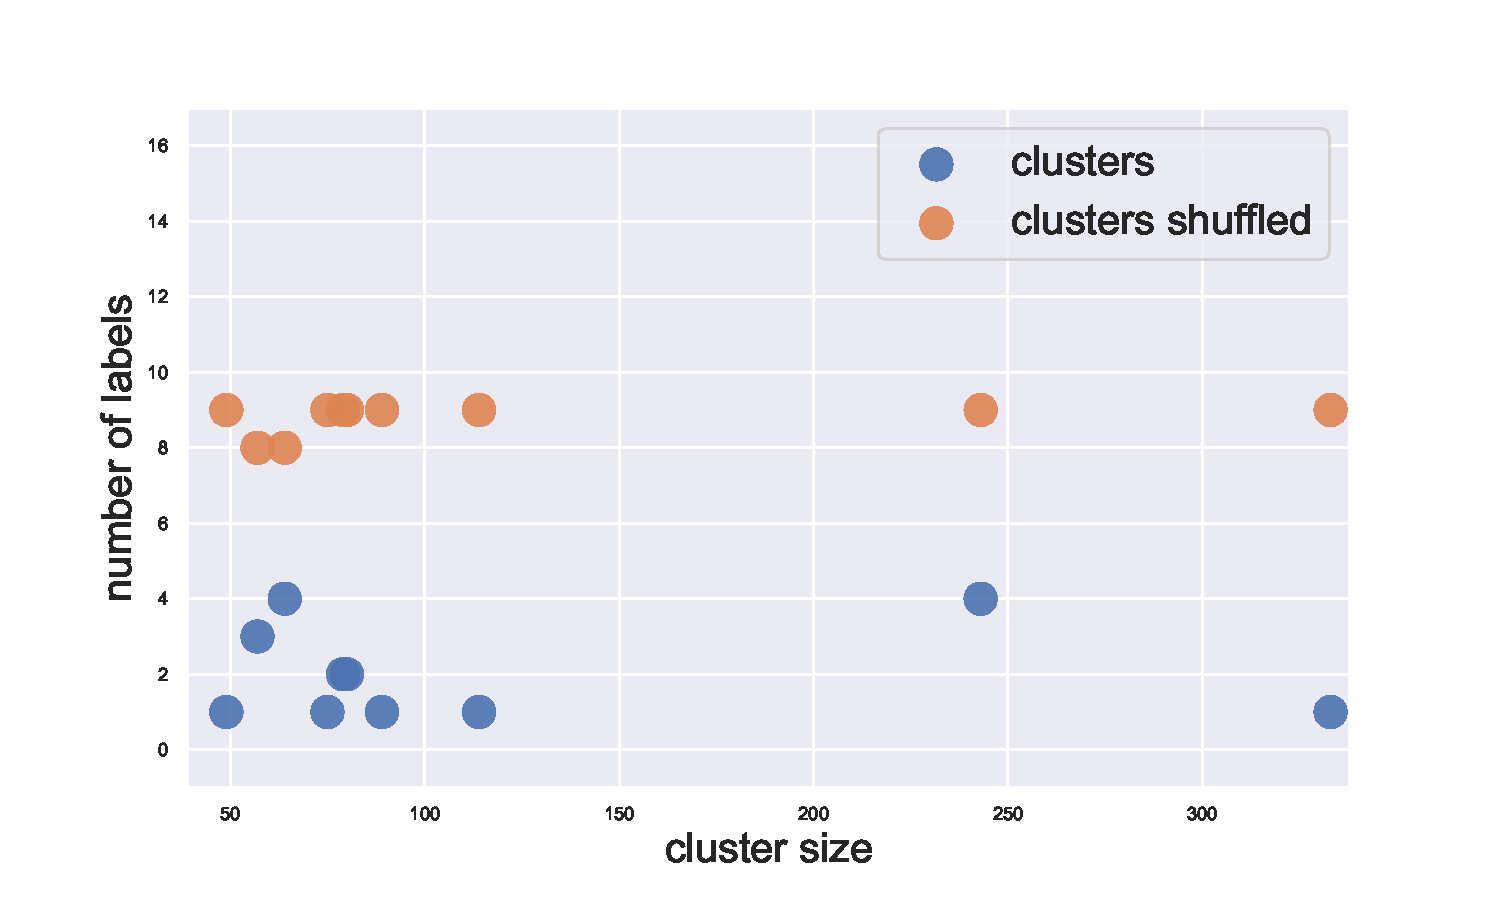
\includegraphics[width=0.9\linewidth]{pictures/topic/gtex/oversigma_10tissue/shuffledcluster_shuffle_label_size_l3_primary_site.pdf}
    \caption{Caption}
    \label{fig:topic/gtex/oversigma_10tissue/shuffledcluster_shuffle_label_size_l3_primary_site}
\end{figure}


\begin{figure}[htb!]
    \centering
    \begin{minipage}{0.45\textwidth}
    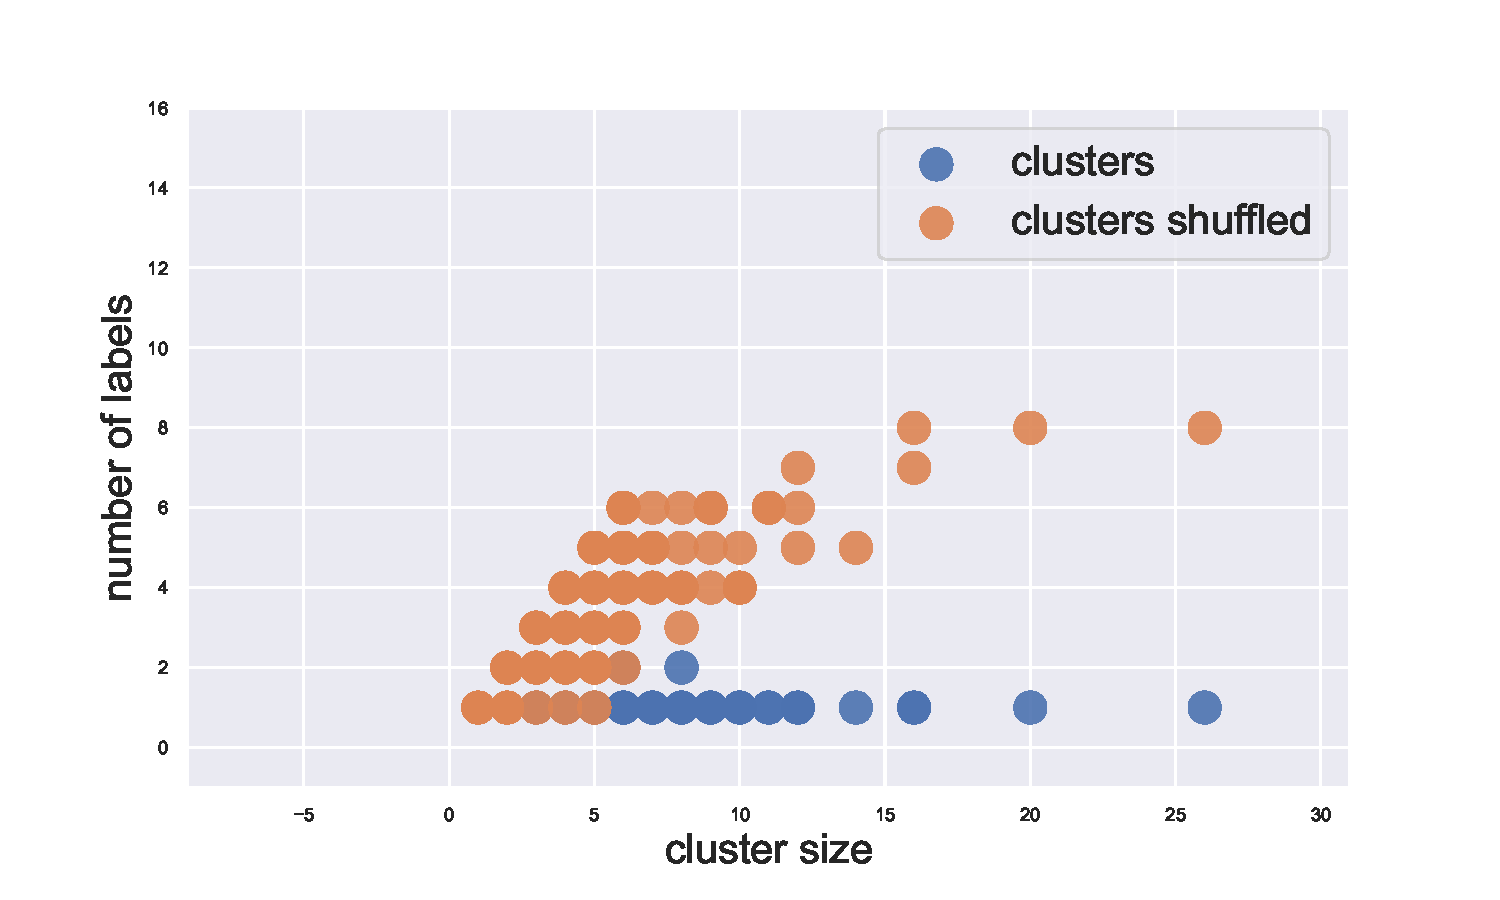
\includegraphics[width=0.9\linewidth]{pictures/topic/gtex/oversigma_10tissue/shuffledcluster_shuffle_label_size_l1_primary_site.pdf}
    \end{minipage}
    \hspace{3mm}
    \begin{minipage}{0.45\textwidth}
    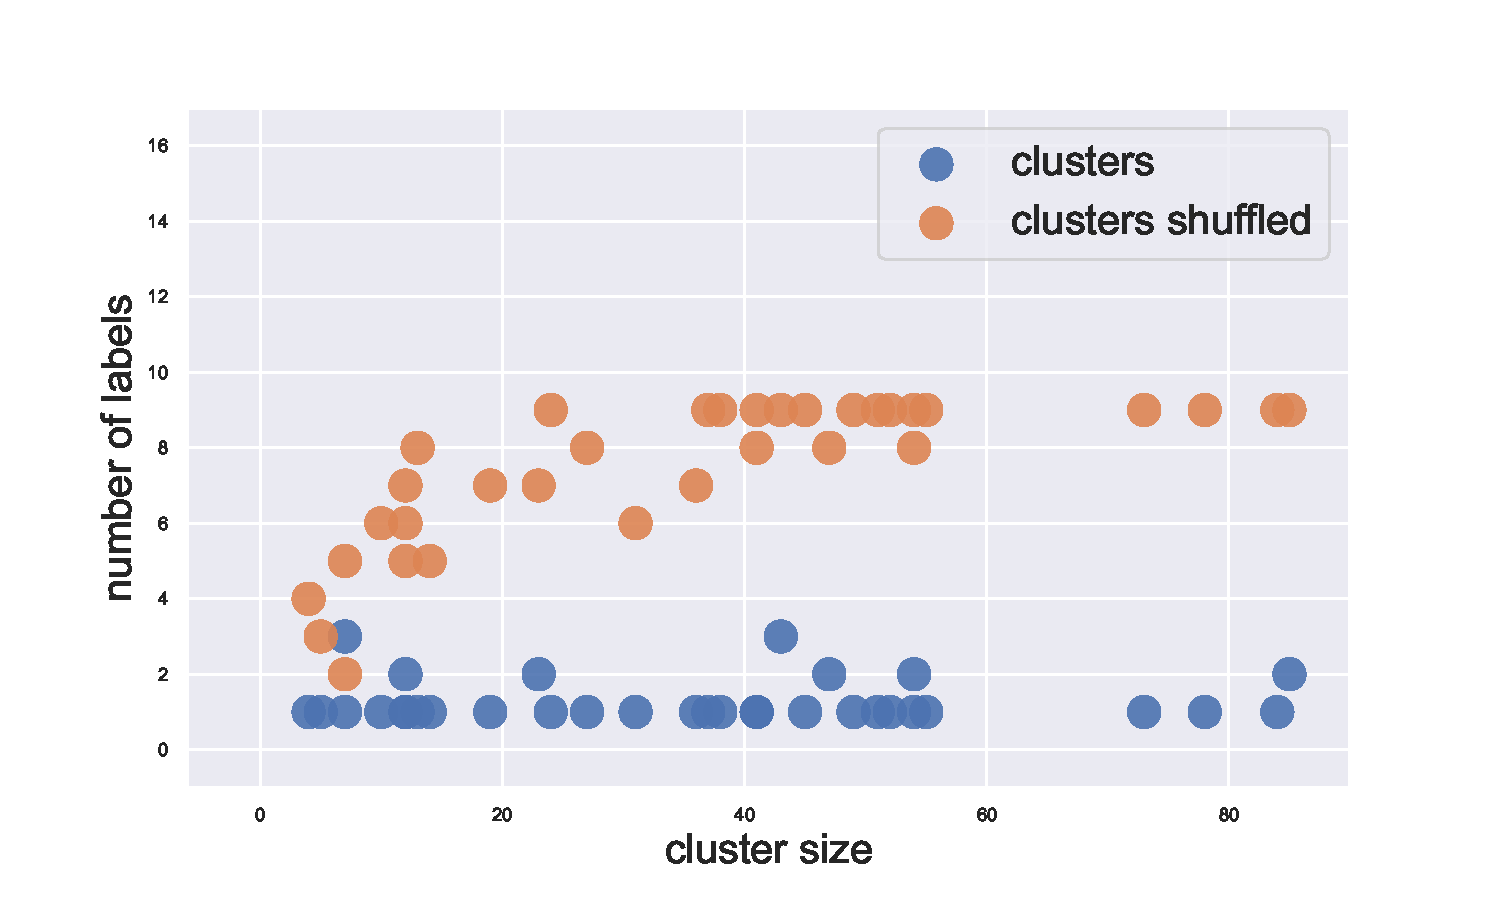
\includegraphics[width=0.9\linewidth]{pictures/topic/gtex/oversigma_10tissue/shuffledcluster_shuffle_label_size_l2_primary_site.pdf}
    \end{minipage}
    \\
    \begin{minipage}{0.45\textwidth}
    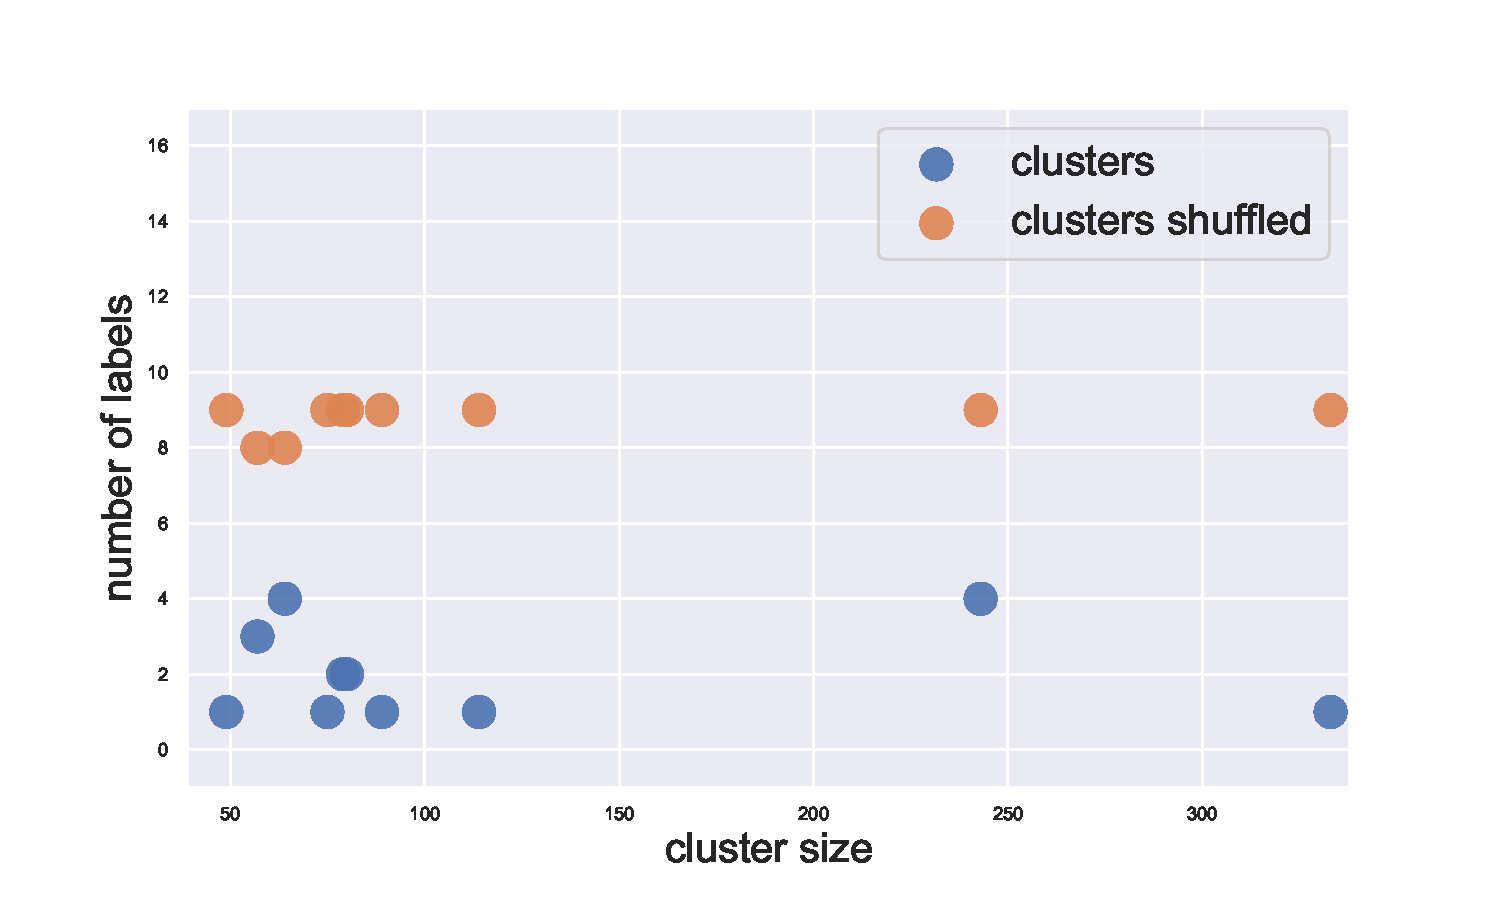
\includegraphics[width=0.9\linewidth]{pictures/topic/gtex/oversigma_10tissue/shuffledcluster_shuffle_label_size_l3_primary_site.pdf}
    \end{minipage}
    \hspace{3mm}
    \begin{minipage}{0.45\textwidth}
    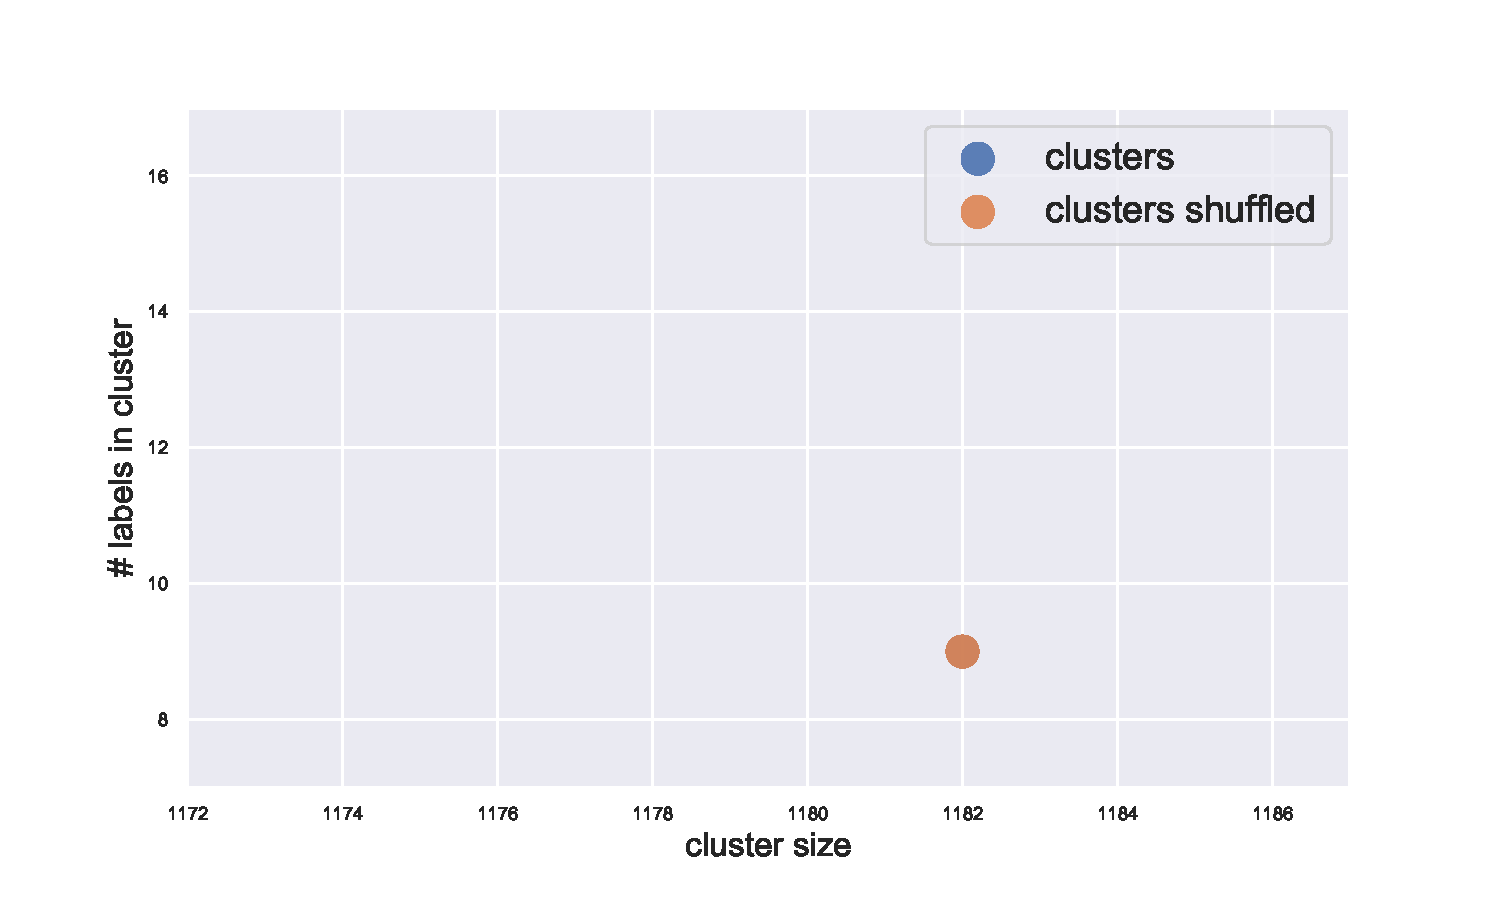
\includegraphics[width=0.9\linewidth]{pictures/topic/gtex/oversigma_10tissue/shuffledcluster_shuffle_label_size_l4_primary_site.pdf}
    \end{minipage}
\end{figure}

\begin{figure}[htb!]
    \centering
    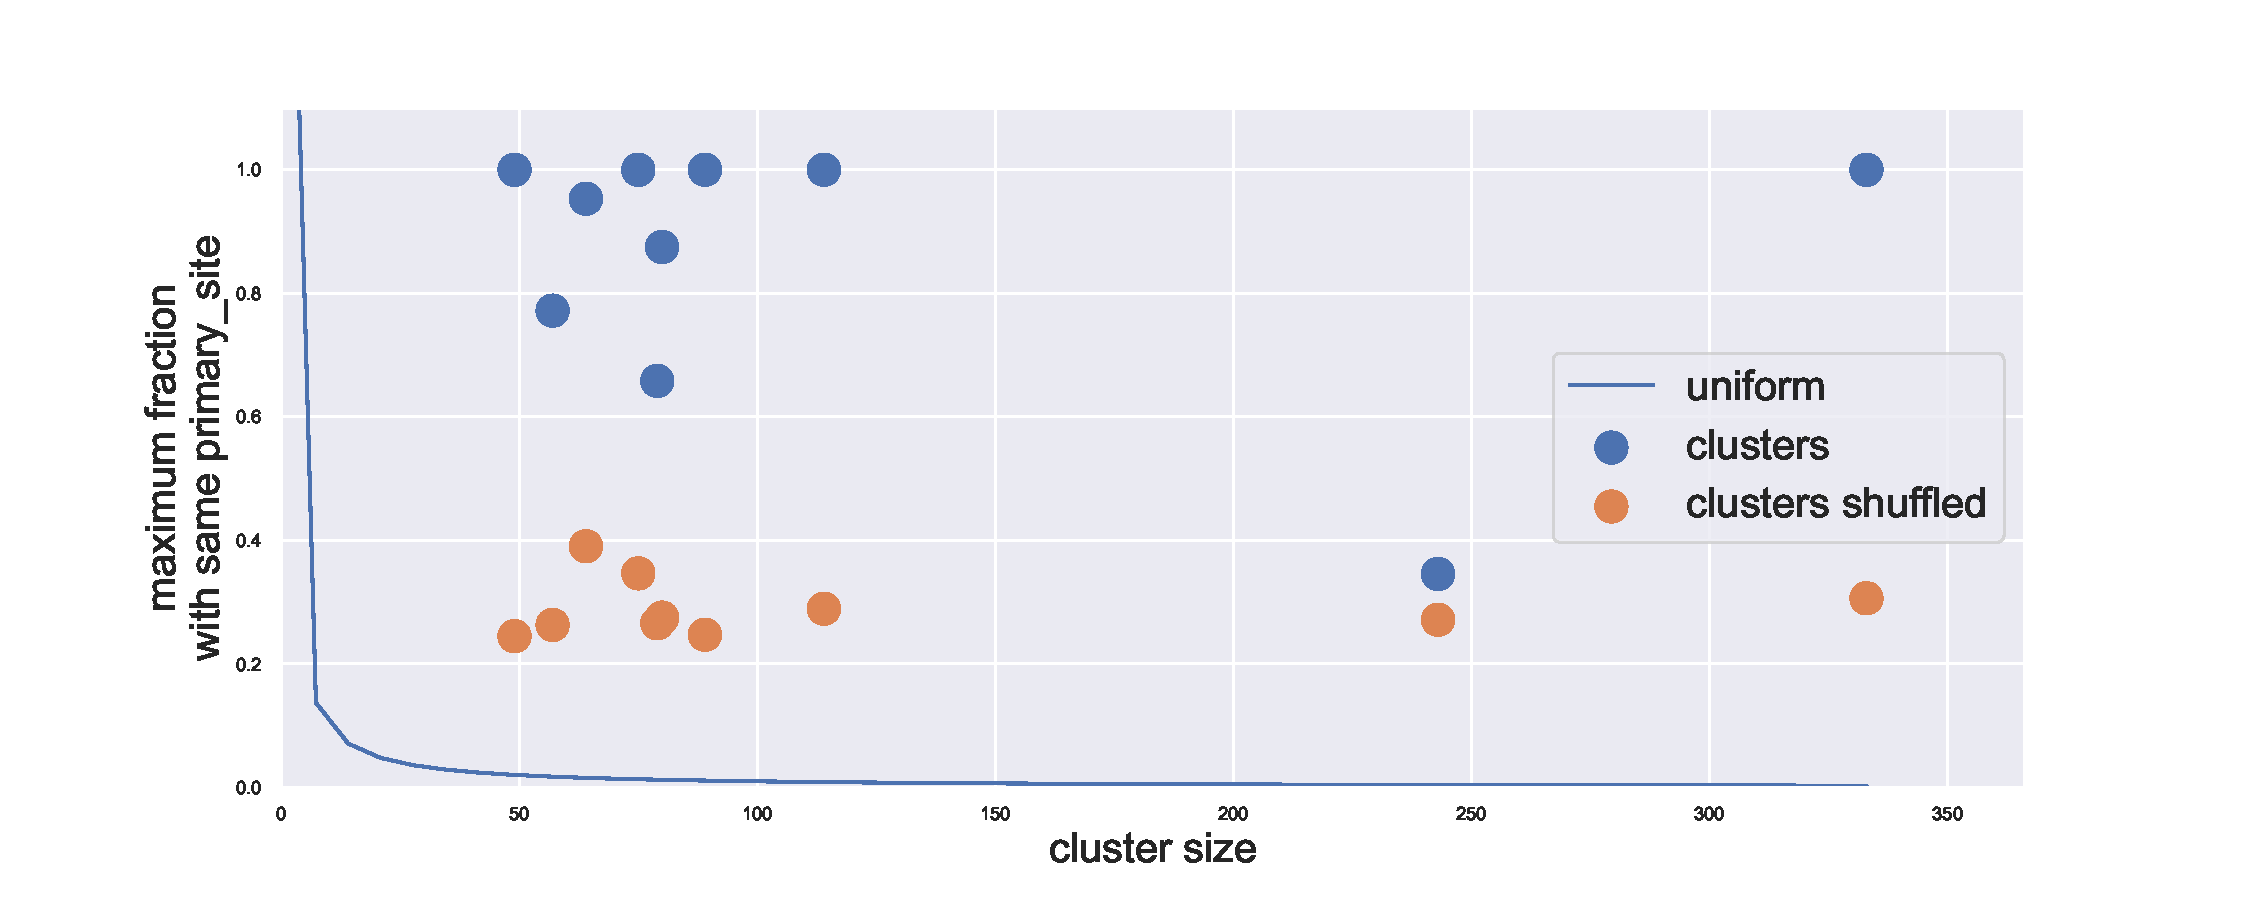
\includegraphics[width=0.9\linewidth]{pictures/topic/gtex/oversigma_10tissue/shuffledclusterhomosize_l3_primary_site.pdf}
    \caption{Caption}
    \label{fig:topic/gtex/oversigma_10tissue/shuffledclusterhomosize_l3_primary_site}
\end{figure}


\begin{figure}[htb!]
    \centering
    \begin{minipage}{0.45\textwidth}
    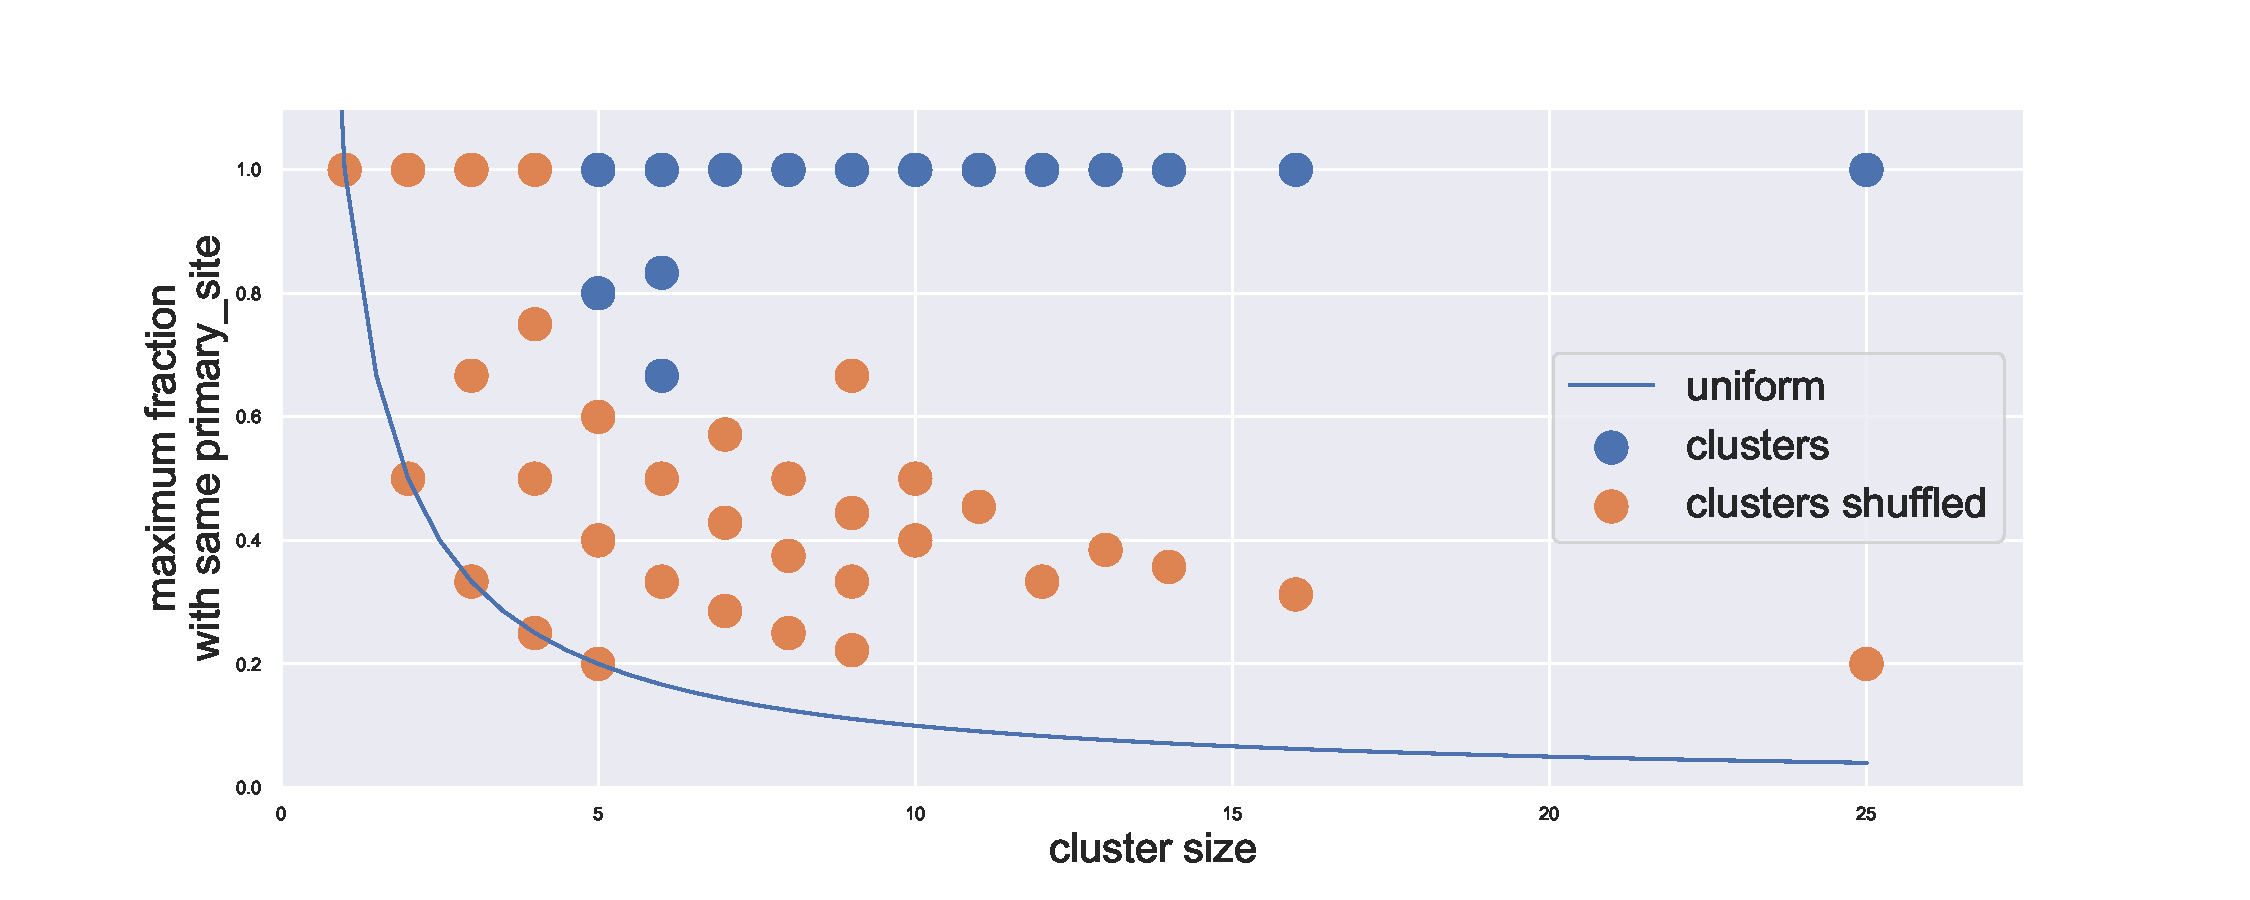
\includegraphics[width=0.9\linewidth]{pictures/topic/gtex/oversigma_10tissue/shuffledclusterhomosize_l1_primary_site.pdf}
    \end{minipage}
    \hspace{3mm}
    \begin{minipage}{0.45\textwidth}
    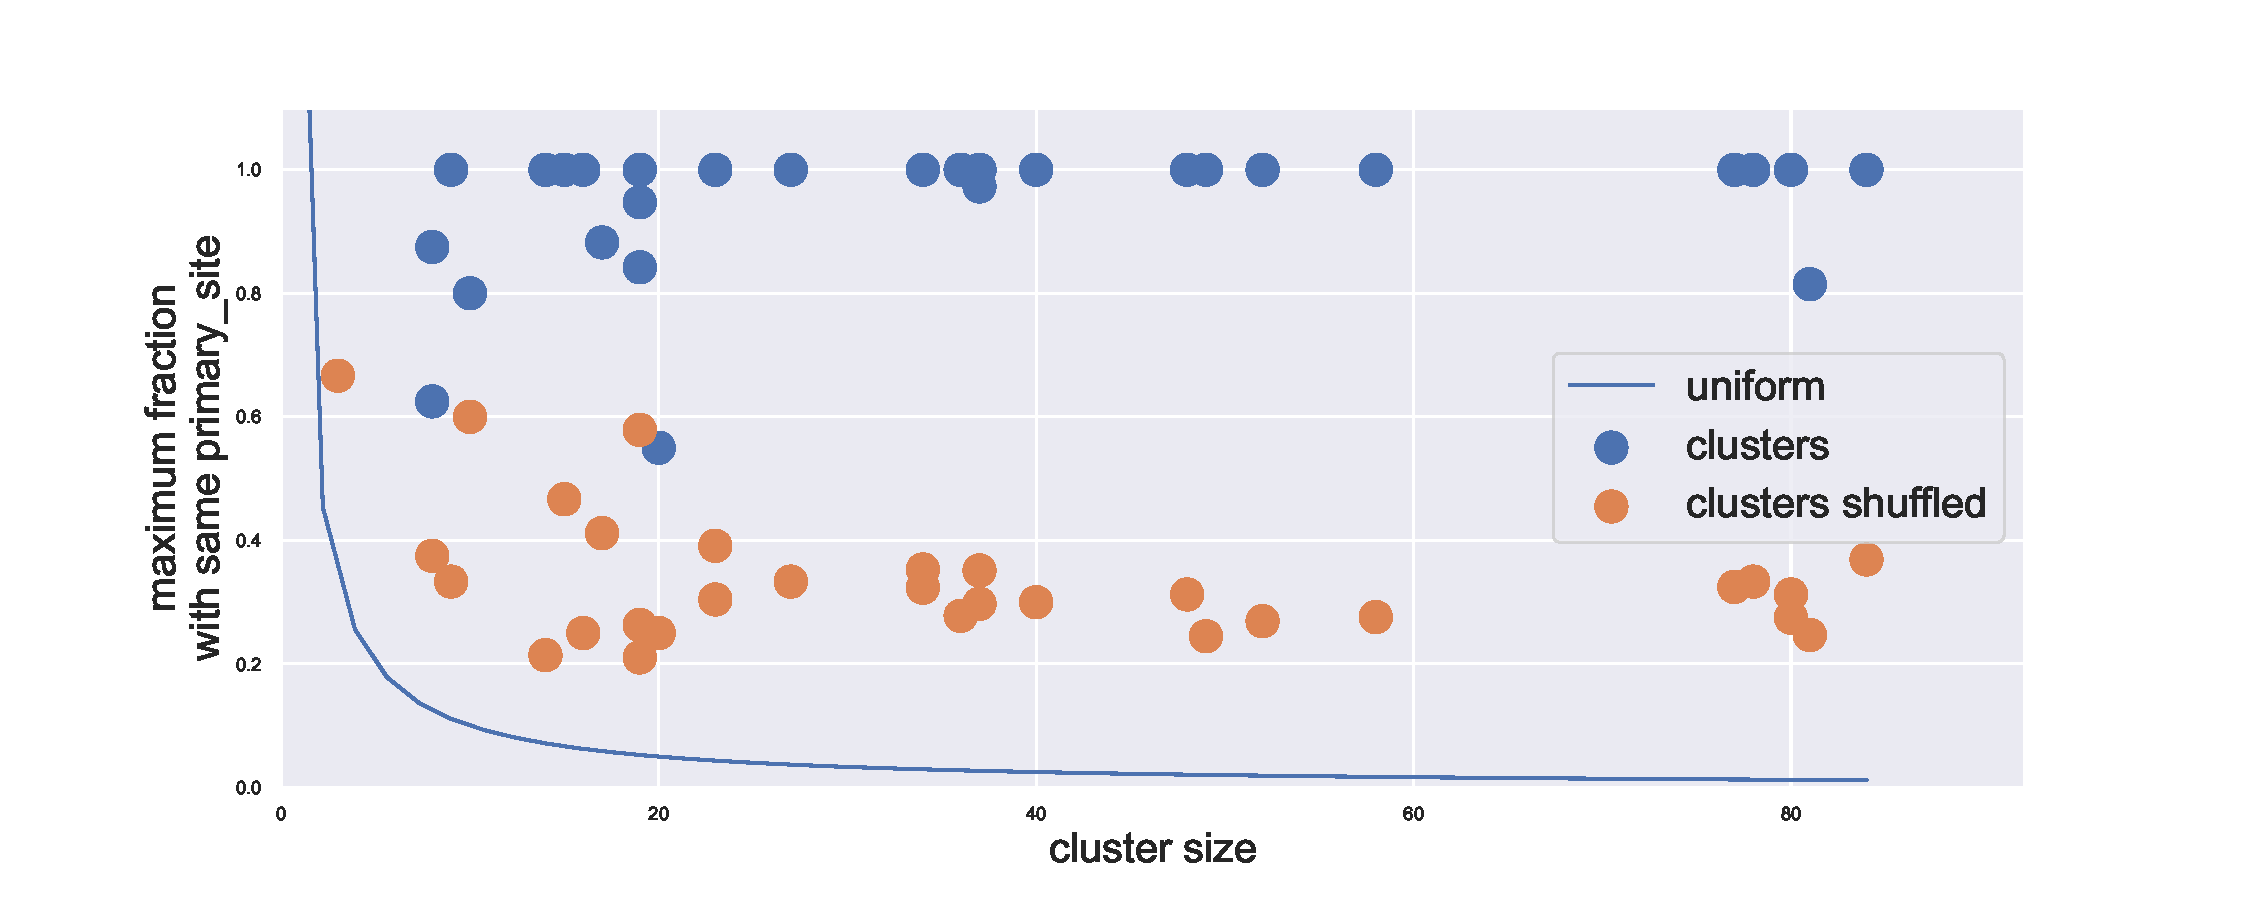
\includegraphics[width=0.9\linewidth]{pictures/topic/gtex/oversigma_10tissue/shuffledclusterhomosize_l2_primary_site.pdf}
    \end{minipage}
    \\
    \begin{minipage}{0.45\textwidth}
    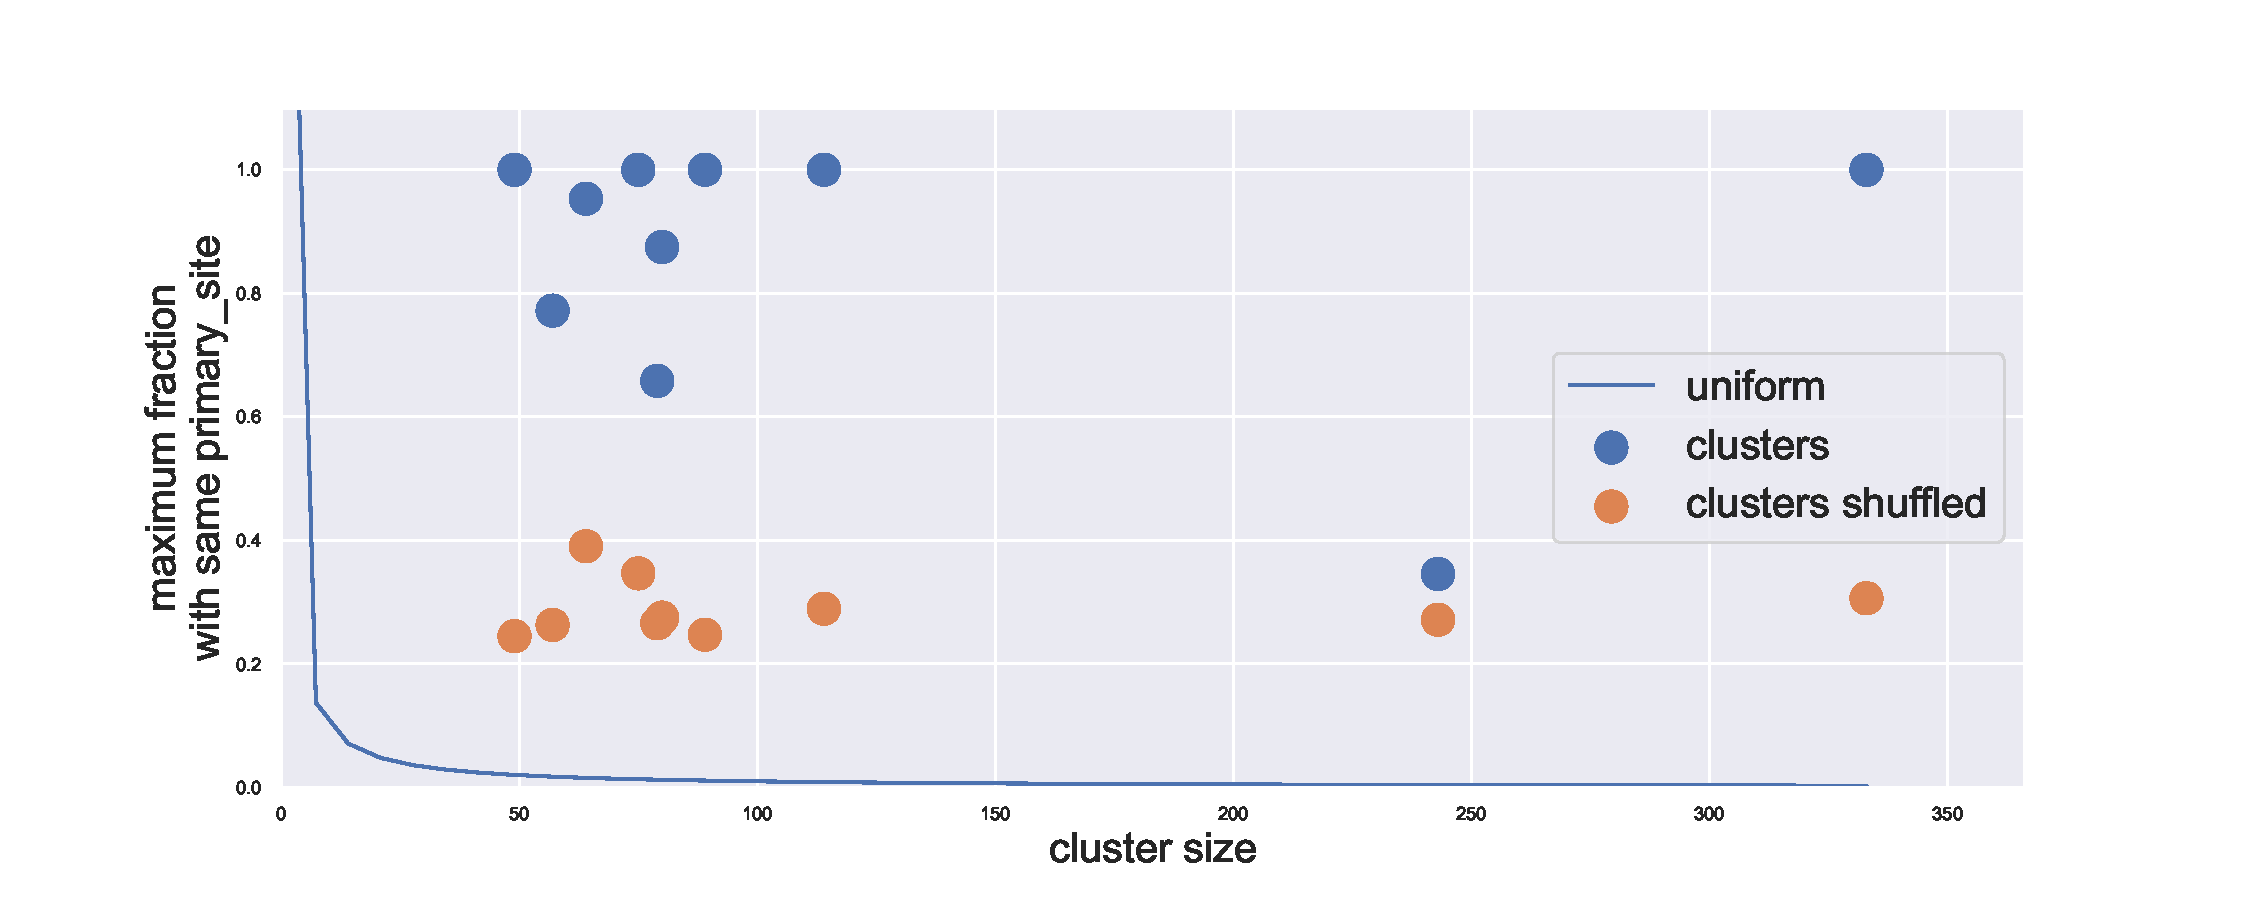
\includegraphics[width=0.9\linewidth]{pictures/topic/gtex/oversigma_10tissue/shuffledclusterhomosize_l3_primary_site.pdf}
    \end{minipage}
    \hspace{3mm}
    \begin{minipage}{0.45\textwidth}
    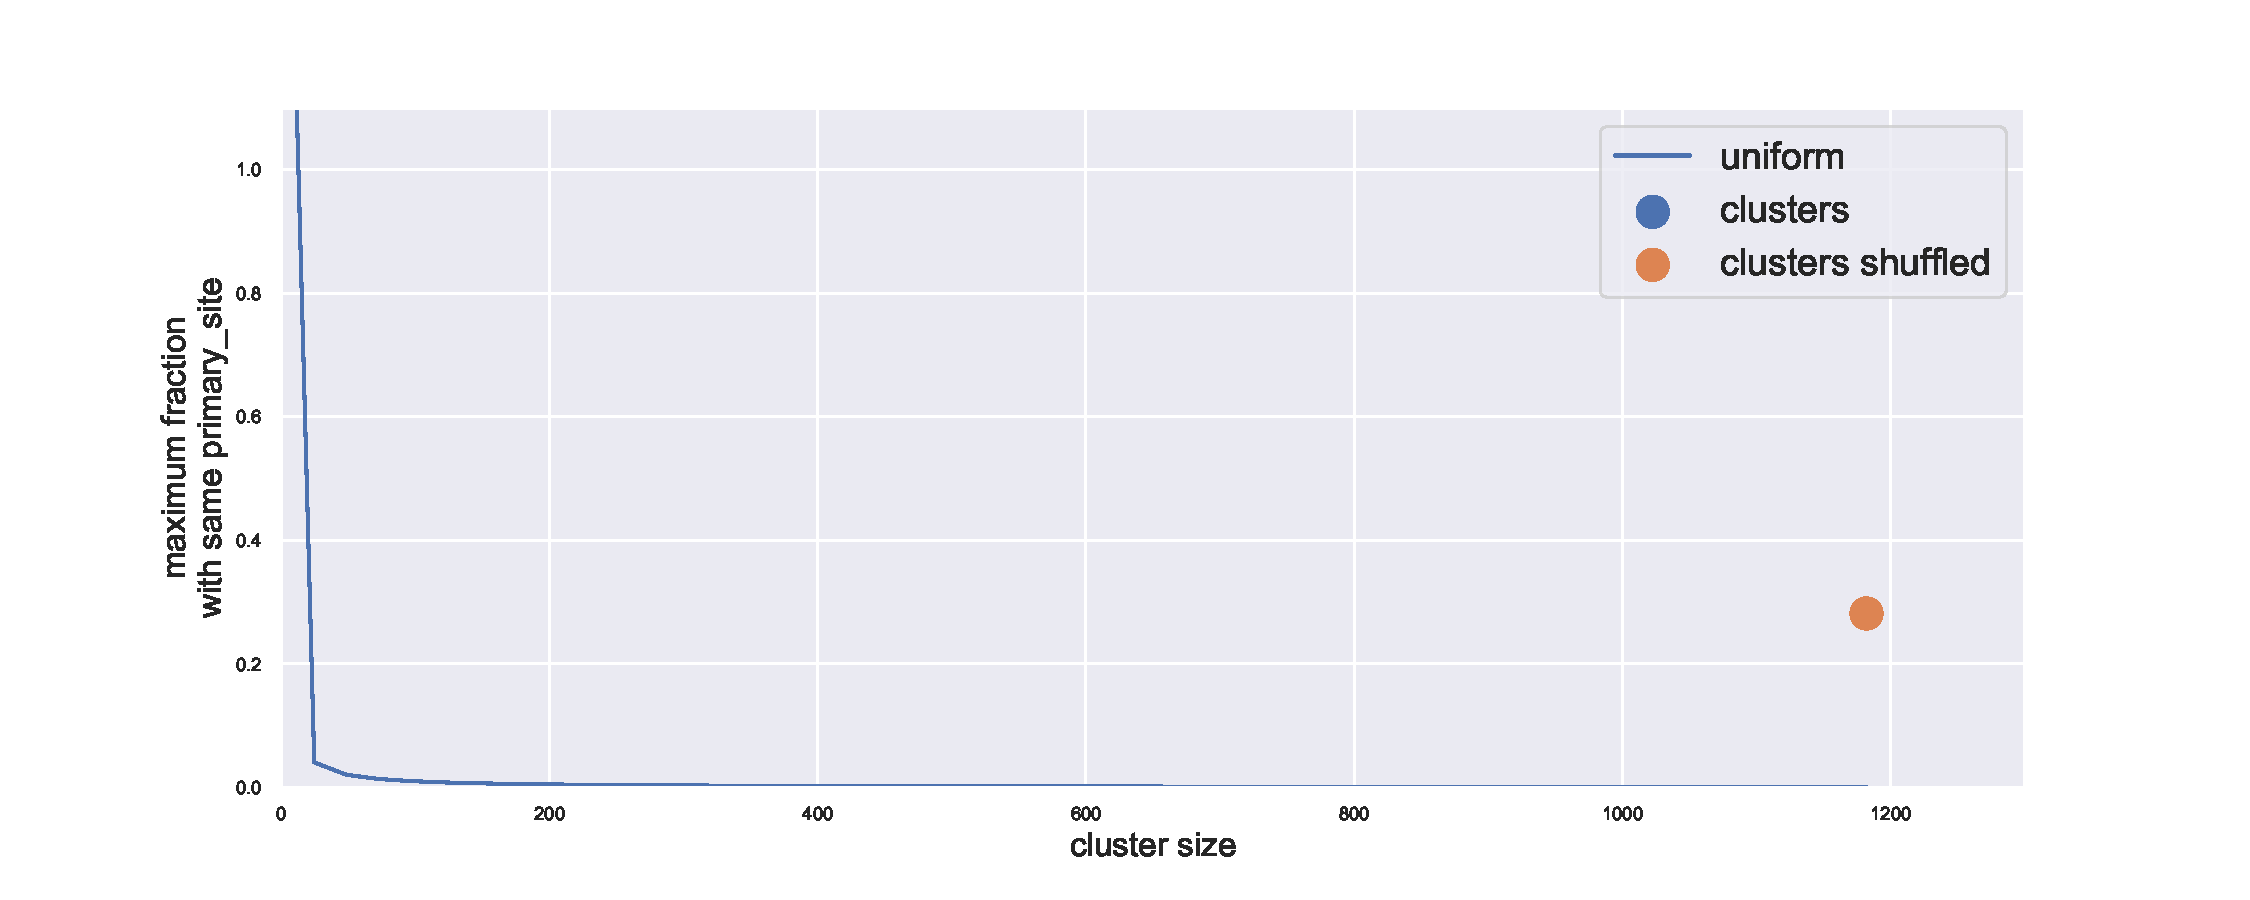
\includegraphics[width=0.9\linewidth]{pictures/topic/gtex/oversigma_10tissue/shuffledclusterhomosize_l4_primary_site.pdf}
    \end{minipage}
\end{figure}


\subsection{Shuffling}

\begin{figure}[htb!]
    \centering
    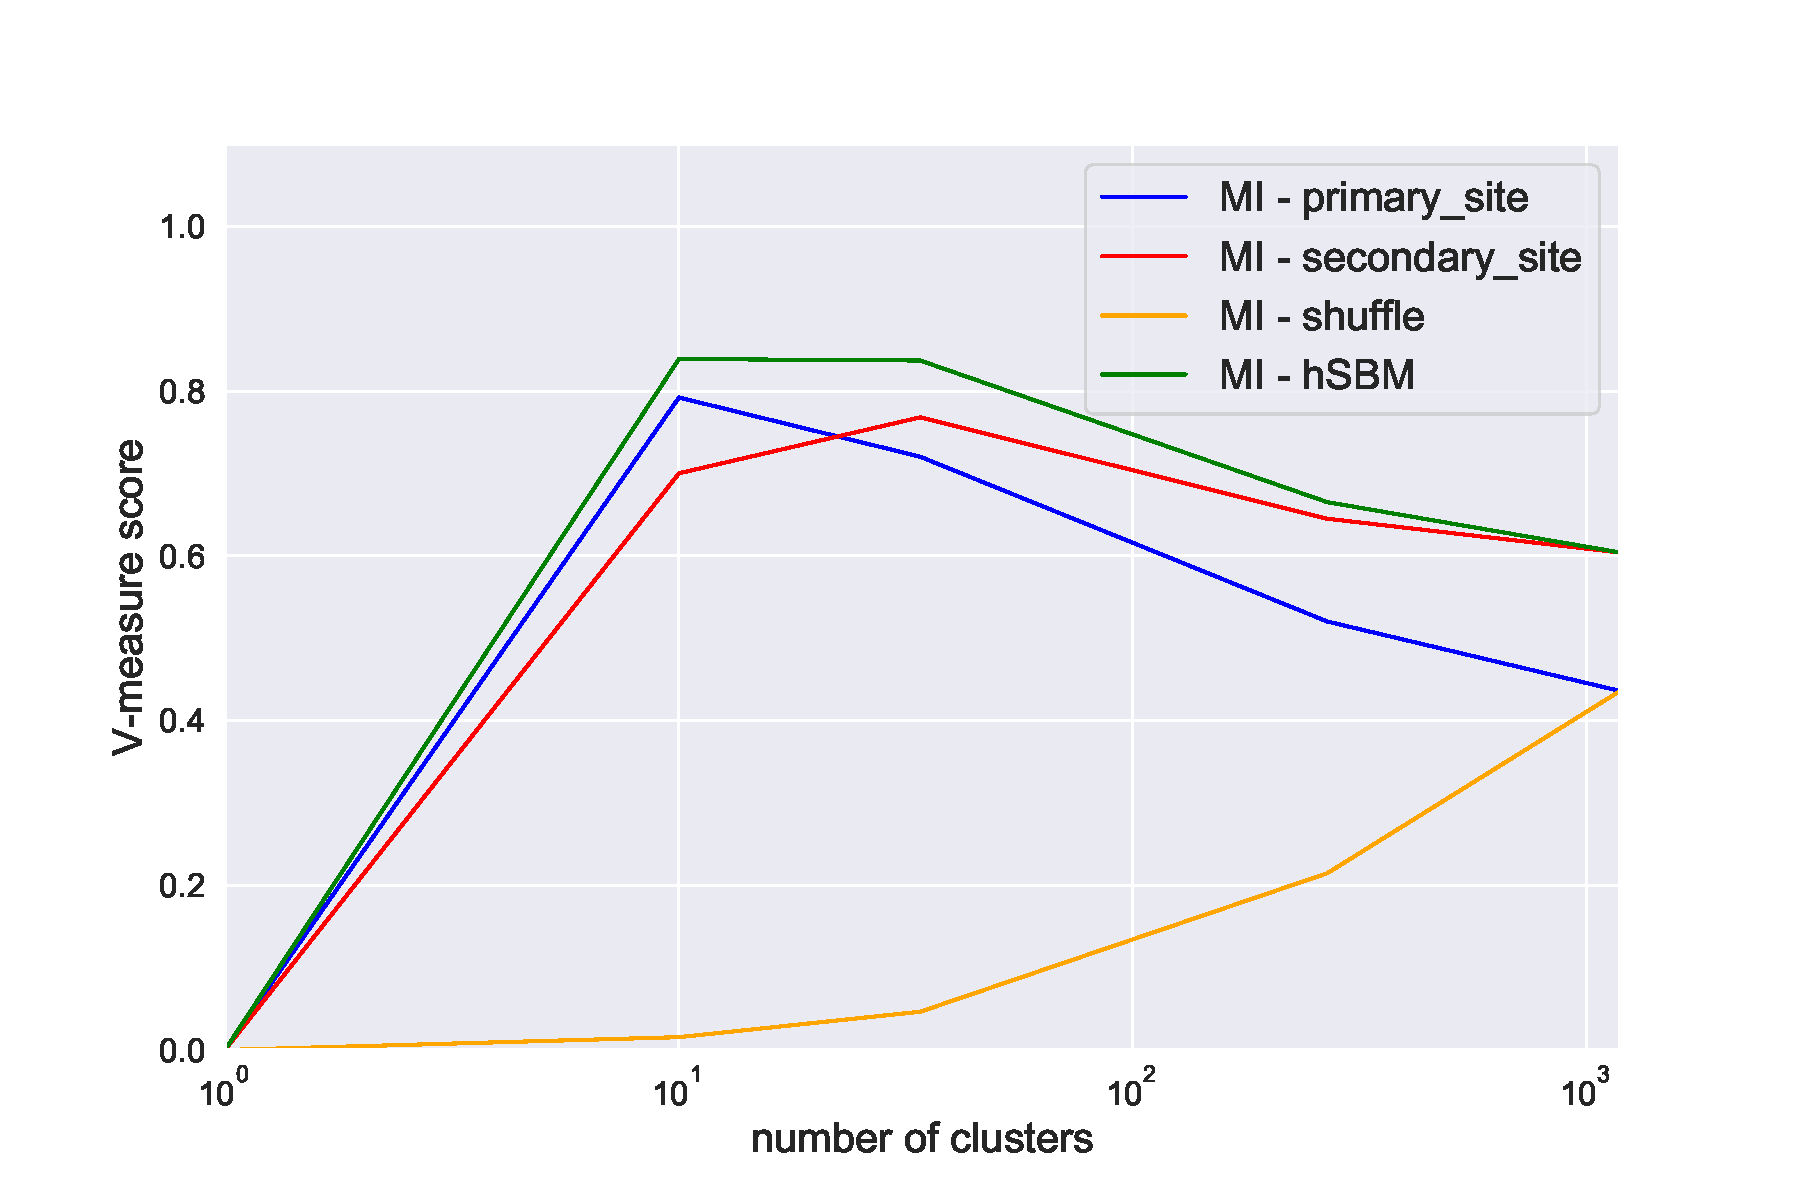
\includegraphics[width=0.9\linewidth]{pictures/topic/gtex/oversigma_10tissue/metric_scores_shuffle.pdf}
    \caption{Scores across hierarchy. The scored is compared with some random labels}
    \label{fig:topic/gtex/oversigma_10tissue/metric_scores_shuffle}
\end{figure}

\subsection{Standard algorithms}

\begin{figure}[htb!]
    \centering
    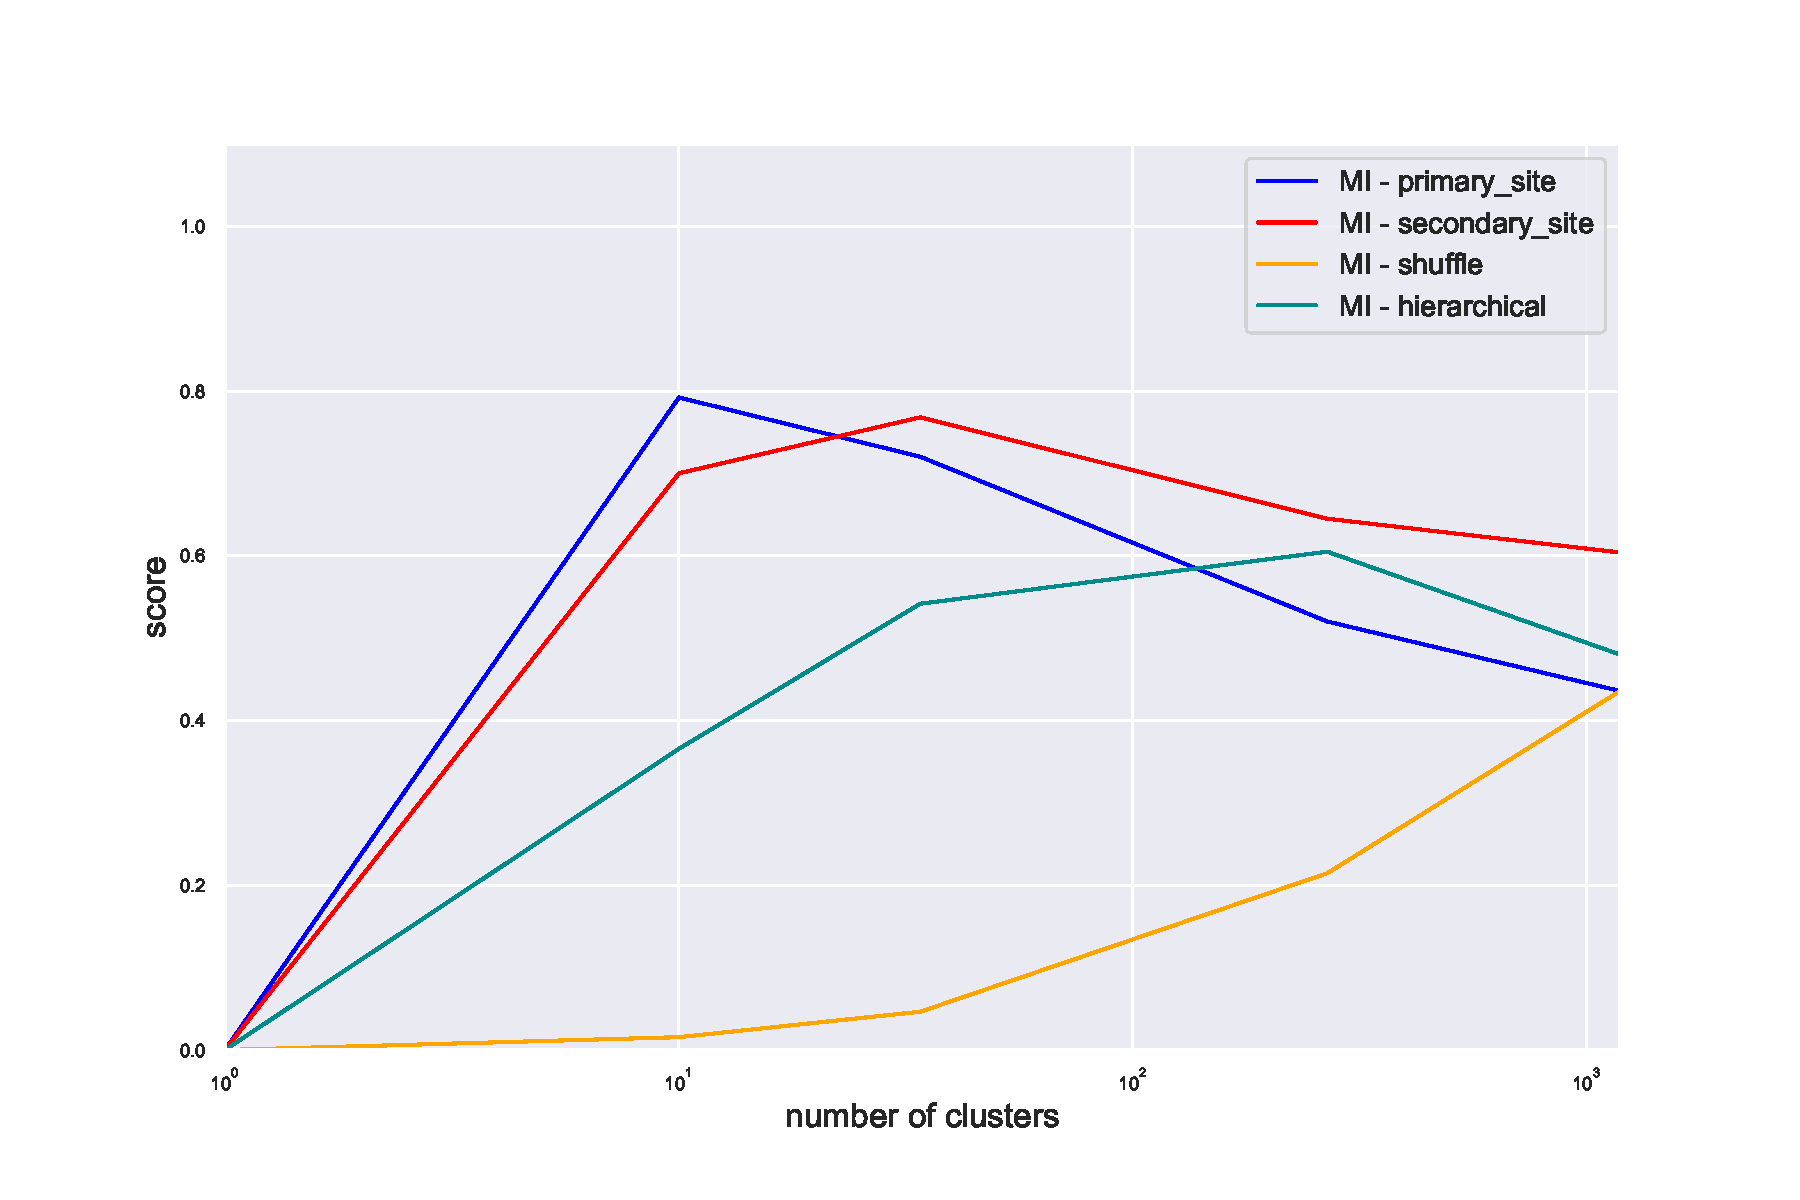
\includegraphics[width=0.9\linewidth]{pictures/topic/gtex/oversigma_10tissue/metric_scores_hier.pdf}
    \caption{Scores across hierarchy. The scored is compared with some random labels}
    \label{fig:topic/gtex/oversigma_10tissue/metric_scores_hier}
\end{figure}

\begin{figure}[htb!]
    \centering
    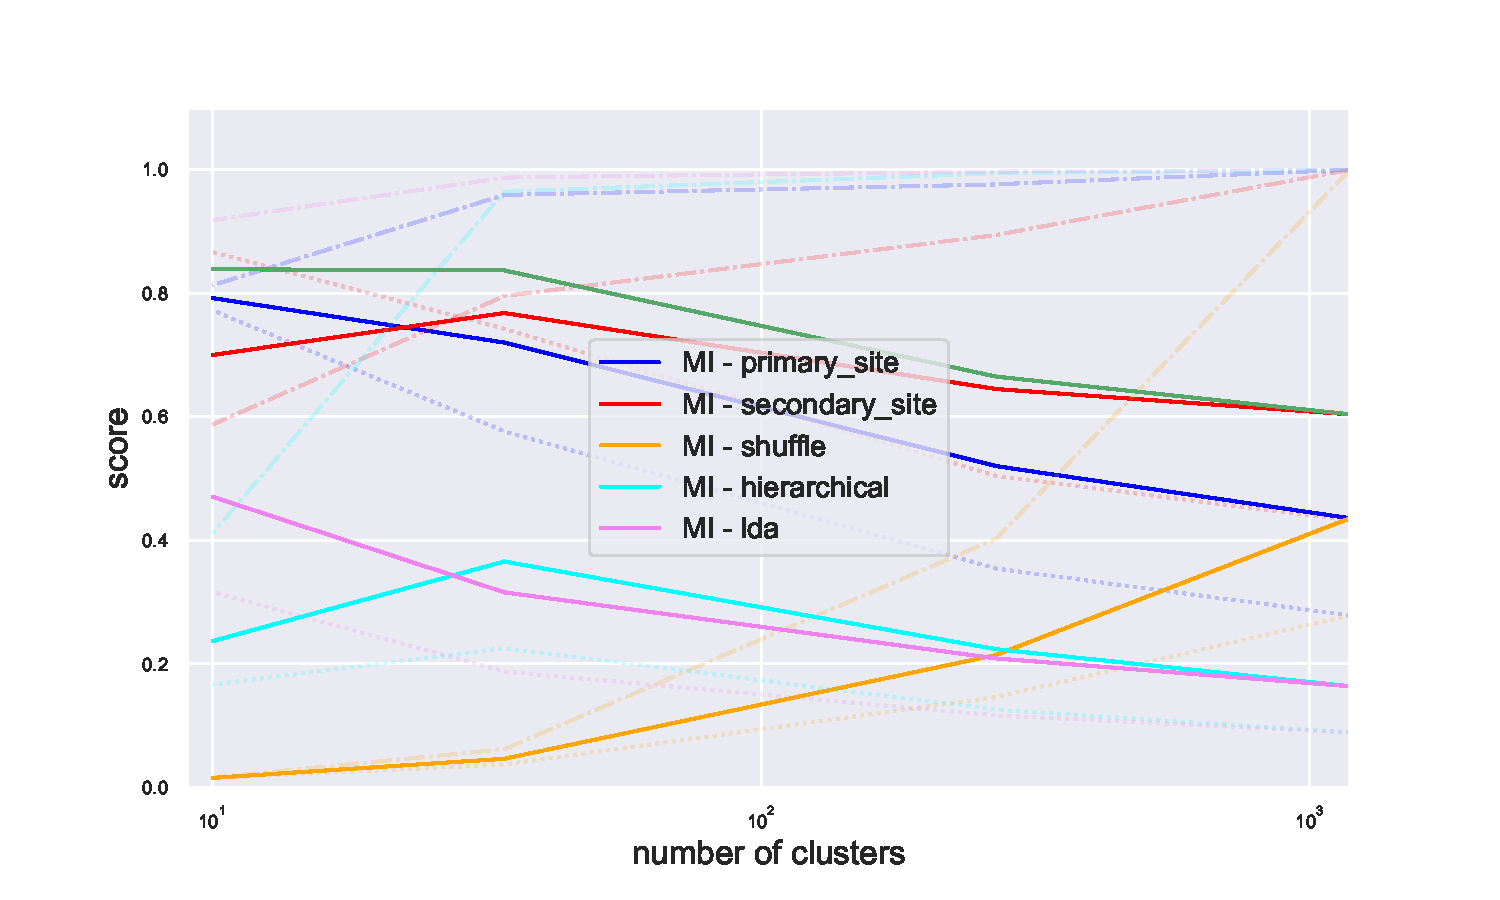
\includegraphics[width=0.9\linewidth]{pictures/topic/gtex/oversigma_10tissue/metric_scores_all.pdf}
    \caption{Scores across hierarchy. The scored is compared with some random labels}
    \label{fig:topic/gtex/oversigma_10tissue/metric_scores_all}
\end{figure}
